%% Copernicus Publications Manuscript Preparation Template for LaTeX Submissions
%% ---------------------------------
%% This template should be used for copernicus.cls
%% The class file and some style files are bundled in the Copernicus Latex Package which can be downloaded from the different journal webpages.
%% For further assistance please contact the Copernicus Publications at: publications@copernicus.org
%% http://publications.copernicus.org


%% Please use the following documentclass and Journal Abbreviations for Discussion Papers and Final Revised Papers.


%% 2-Column Papers and Discussion Papers
\documentclass[gmd, manuscript, draft]{copernicus}

%% Journal Abbreviations (Please use the same for Discussion Papers and Final Revised Papers)
% Geoscientific Model Development (gmd)

%% \usepackage commands included in the copernicus.cls:
%\usepackage[german, english]{babel}
%\usepackage{tabularx}
%\usepackage{cancel}
%\usepackage{multirow}
%\usepackage{supertabular}
%\usepackage{algorithmic}
%\usepackage{algorithm}
%\usepackage{amsthm}
\usepackage{amsmath}
\usepackage{bm}
\usepackage{siunitx}
%\usepackage{float}
%\usepackage{subfig}
%\usepackage{rotating}
\usepackage{subcaption}

\newcommand{\matr}[1]{\mathbf{#1}}
\usepackage{color}

\begin{document}

\linenumbers

\title{EcoGEnIE 0.1: Plankton Ecology in the cGENIE Earth system model}


\Author[1,2]{}{B. A.~Ward}
\Author[1]{}{J. D.~Wilson}
\Author[1]{}{R.~De'Ath}
\Author[1]{}{F.~Monteiro}
\Author[2]{}{A.~Yool}
\Author[1,3]{}{A.~Ridgwell}

\affil[1]{\small{School of Geographical Sciences, University of Bristol, Bristol BS8 1SS, UK}}
\affil[2]{\small{National Oceanography Centre, European Way, Southampton SO14 3ZH, UK}}
\affil[3]{\small{Department of Earth Sciences, University of California, Riverside CA, USA}}
%% The [] brackets identify the author with the corresponding affiliation. 1, 2, 3, etc. should be inserted.


        
\runningtitle{~}

\runningauthor{B.A. Ward \textit{et al.}}

%\correspondence{Ben Ward (b.a.ward@bristol.ac.uk)}



\received{}
\pubdiscuss{} %% only important for two-stage journals
\revised{}
\accepted{}
\published{}

%% These dates will be inserted by Copernicus Publications during the typesetting process.


\firstpage{1}

\maketitle



\begin{abstract}
We present an extension to the cGENIE Earth System model that explicitly accounts for the growth and interaction of an arbitrary number of plankton species. The new  package (`ECOGEM') replaces the implicit, flux-based, parameterisation of the plankton community currently employed, with explicitly resolved plankton populations and ecological dynamics. In ECOGEM,  any number of plankton species, with ecophysiological traits (e.g. growth and grazing rates) assigned according to organism size and functional group (e.g. phytoplankton and zooplankton) can be incorporated at run-time. We illustrate the capability of the marine ecology enabled Earth system model (`EcoGENIE') by comparing results from one configuration of ECOGEM (with eight generic phytoplankton and zooplankton size classes) to climatological and seasonal observations. We find that the new ecological components of the model  show reasonable agreement with both global-scale climatological and local-scale seasonal data. We also compare  EcoGENIE results to the existing biogeochemical incarnation of cGENIE. We find that the resulting global-scale distributions of phosphate, iron, dissolved inorganic carbon, alkalinity and oxygen are similar for both iterations of the model.  A slight deterioration in some fields in EcoGENIE, relative to the data is observed,  although we make no attempt to re-tune the overall marine cycling of carbon and nutrients   here.  The increased capabilities of EcoGENIE in this regard will enable future exploration of the ecological community on much longer timescales than have previously been examined in global ocean ecosystem models and particularly for past climates and global biogeochemical cycles.
\end{abstract}

%\clearpage
%\small{
%\tableofcontents*}
%\clearpage

%%%%%%%%%%%%%%%%%%%%%%%%%%%%%%%%%%%%%%%%%%%%%%%%%%%%%%%%%%%%%%%%%%%%%%%
%%%%%%%%%%%%%%%%%%%%%%%%%%%%%%%%%%%%%%%%%%%%%%%%%%%%%%%%%%%%%%%%%%%%%%%
\introduction  %% \introduction[modified heading if necessary]

The marine ecosystem is an integral component of the Earth system and its dynamics. Photosynthetic plankton ultimately support almost all life in the ocean, including the the fisheries that provide essential nutrition to more than half the human population \citep{Hollowed:2013}. In addition, the oceans provide a key sink for carbon released into the atmosphere, playing a key role in moderating the climate. The strength of this sink, in turn, is modulated by the activity and composition of marine ecosystems and how this controls the `biological pump' in the ocean.  (The biological pump constitutes the  photosynthetic uptake of carbon  in the well-lit ocean surface, followed by the downward transport and deep remineralisation of organic matter, resulting in a net increase in in the partial pressure of CO$_2$ at depth and decrease in the ocean surface and atmosphere -- see \textcolor{red}{H\"uelse et al. [in revision]}.) For instance, the existence of the biological carbon has been estimated to equate to a reduction in atmospheric carbon concentration at steady state of approximately 200 ppm \citep{Parekh:2006}, with variations in its magnitude being cited as playing a key role, for example, in the late Quaternary glacial-interglacial climate oscillations \citep{Hain:2014} [\textcolor{red}{ Watson et al., 2000}].

A variety of different marine biogeochemical modelling approaches have been developed in an attempt to understand  how the marine carbon cycle functions and its dynamical interaction with climate, and to make both past and future projections. In the  simplest of these approaches, the  biological pump is incorporated into an ocean circulation (or box) model without  explicitly   including any state-variables for  the biota. Such models have been described as models of `biogenically induced chemical fluxes' (rather than explicitly of the biology (and ecology) itself) \citep{Maier-Reimer:1993}. They vary considerably in complexity, but can be broadly divided into two categories. In the first of these --  `nutrient-restoring' -- models calculate the biological uptake of nutrients at any one point at the ocean surface as the flux required to  maintain surface nutrient concentrations at observed values \cite[e.g.][]{Bacastow:1990,Najjar:1992}. The vertical flux is then remineralised at depth according to some attenuating profile, such as that of \citet{Martin:1987}.  Within this framework, carbon export is typically calculated from the nutrient flux according to a fixed stoichiometric (`Redfield') ratio. In addition to the availability of a spatially explicit (in the case of ocean circulation models)  observed surface ocean nutrient field, nutrient restoring models inherently only require a single parameter -- the restoring time-scale, and even this parameter is not critical (as long as the time-scale is sufficiently short that the model closely reproduces the observed nutrient concentrations). The simplicity of this approach lends itself to being able to focus on a very specific part of the ecosystem dynamics, namely the downward transport of organic matter, and was highly influential particularly during the early days of  marine biogeochemical  model development and  assessment of carbon uptake and transport dynamics (e.g. \textcolor{red}{Marchal et al. [1998], Najjar et al. [1992]}). However, because this approach is based explicitly upon  observed values (or modified observations), they are  primarily only suitable for diagnostic and modern steady-state applications and are unable to model any deviations in nutrient cycling and hence climate from the current ocean state. 

More sophisticated models of biogenically induced chemical fluxes do away with a direct observational constraint and instead estimate the organic matter export term on the basis of limiting factors, such as temperature, light and the availability of nutrients such as nitrogen, phosphorous and iron -- an approach we will here refer to as   `nutrient-limitation'. Models based on this approach  (e.g. Bacastow and Maier-Reimer, 1990; Henze et al., 1991; Archer and Johnson, 2000)  were natural successors to the early nutrient restoring models and could account for the influence of multiple limiting nutrients and even implicitly partition export between different functional types (e.g.; Watson et al., 2000). Without entraining an explicit dependence on observed surface ocean nutrient distributions, these  models also now gain much more freedom and with it, a degree of predictive capability.  Additionally, other than plausible values for nutrient half-saturation constants, nutrient-limitation models make few assumptions that are specifically tied to modern observations, and assume very little (if anything) about the particular organisms present. Hence, as long as one makes the assumption that the marine plankton that existed at some specific time in the past were   physiologically similar, particularly in terms of fundamental nutrient requirements, there is no  apparent reason why nutrient-limitation models will not be as applicable to much of the Phanerozoic in terms of geological past, as they are to the present (questions of how suitable they might be to the present in the first place, aside). Using nutrient-limitation flux schemes, marine biogeochmcial cycles have hence already been simulated for periods such as the early Eocene [\textcolor{red}{REF}], mid and late Cretaceous [\textcolor{red}{REF}], and end Permian [\textcolor{red}{REF}], times when surface nutrient distributions are not known \textit{a priori}.

The disadvantage of both  variants  of models of biogenically induced chemical fluxes, is that they are not able to represent interactions between parts of the ecosystem (e.g. resource competition and predator-prey interactions), simply because these processes are not resolved. Nor can they address questions involving the addition or loss, such as associated with past extinction events, of plankton species and changes in ecosystem complexity and/or structure. They also suffer from being overly responsive to changes in nutrient availability. In the case of restoring models this is simply because any change in the target field will be closely tracked. In the case of the nutrient-limitation models,  the lack of an explicit biomass term  results in export fluxes  changing instantaneously in response to changing limiting factors. In contrast, in the real world,  sufficient biomass must first exist, such as in a bloom condition, in order to achieve maximal export. This has consequences for the how the seasonality of organic matter  export  is represented. Other restrictions include the inability to know anything about ecosystem size structure (and, by association, about particle sinking speed), or the degree of recycling at the ocean surface and hence the partitioning of carbon into dissolved vs. particulate phases in exported organic matter. 

To allow models to respond to changes in ecosystem structure, and to incorporate some of the additional  feedbacks and complexities that may be important in determining the future marine response to continued greenhouse gas emissions [\textcolor{red}{REF -- e.g. LeQuere or Bopp ?}], it has been necessary to explicitly resolve the ecosystem itself. Such models have been developed across a wide range of complexities \citep{Kwiatkowski:2014}. Among the simplest are `NPZD' type models, resolving a single nutrient, homogenous  phytoplankton and zooplankton communities, and a single detrital pool \citep{Wroblewski:1988,Oschlies:2001}. At the other end of the spectrum, more complex models may include multiple nutrients and several `Plankton Functional Types' (PFTs) \citep[e.g.][]{Aumont:2003,Moore:2002,LeQuere:2005}. What links these models is that the living state variables are very broadly based on ecological guilds (i.e. groups of organisms that exploit similar resources). 

While simple models have been shown to be capable of reproducing the bulk properties of ecosystems on both regional and global scales \citep{Palmer:2001,Spitz:2001,Schartau:2003pt2,Anderson:2005} many important biogeochemical processes and climate feedbacks can only be resolved by more complex models \citep{LeQuere:2005,Hood:2006}. Additionally, as the composition of the broad ecological guilds used to define NPZD models will be subject to change through both time and space, PFT models may be more generally applicable because they resolve relatively more fundamental ecological components \citep{Friedrichs:2007}. These are the key motivations behind the development of PFT models, in which the broad categories of the NPZD models are replaced with more specific groups based on biogeochemical function. By resolving these key actors in the system, it is possible for the models to capture important climate feedbacks that cannot be represented in simpler models \citep{LeQuere:2005}. 

However, alongside their advantages, the current generation of PFT models are faced with two important and conflicting challenges. Firstly, these complex models contain a large number of parameters that are often poorly constrained by observations \citep{Anderson:2005}. Secondly, although PFT models resolve more ecological structure than the preceding generation of ocean ecosystem models, they are rarely general enough to perform well across large environmental gradients \citep{Friedrichs:2006,Friedrichs:2007,Ward:2010}. To these, one might add difficulties in their application to past climates. PFT models are based on a conceptual reduction of the modern marine ecosystem to its apparent key biogeochemical components, such as nitrogen fixation, or opal frusicle production (as by diatoms). The role of diatoms and the attendant cycling of silica quickly becomes moot once one looks back in Earth history as diatoms only evolved during the Mesozoic and did not proliferate and come to a modern-like dominance until later in the Cenozoic [\textcolor{red}{REFS}]. In addition, the physiological details of each species encoded in the model
are  taken directly from laboratory culture experiments of isolated strains [Le Quere et al., 2005] creating a parameter-dependence on the modern (\textit{in vitro}) ecosystem, in addition to a structural one. 

Recent studies have begun to address these issues by focussing on the more general rules that govern diversity (rather than by trying to quantify and parameterise the diversity itself). These `trait-based' models are beginning to be applied in the field of marine biogeochemical modelling \citep[e.g.][]{Follows:2007,Bruggeman:2007}, with a major advantage being that they are able to resolve greater diversity with fewer specified parameters. One of the main challenges of this approach then is to identify the general rules or trade-offs that govern competition between organisms \citep{Follows:2007,Litchman:2007}. These trade-offs are often strongly constrained by organism size. A potentially large number of different plankton size classes can therefore be parameterised according to well known allometric relationships linking plankton physiological traits to organism size \citep[e.g.][]{Tang:1995,Hansen:1997a}. This approach has the associated advantage that the size composition of the plankton community affects the biogeochemical function of the community \citep[e.g.][]{Guidi:2009}. If one assumes that the same allometric relationships and trade-offs are relatively invariant with time, then this approach provides a potential way forward to addressing geological questions. 

In this paper we present an adaptable modelling framework with an ecological structure that can be easily adapted according to the scientific question at hand. The model is formulated so that all plankton are described by the same set of equations, and any differences are simply a matter of parameterisation. Within this framework, each plankton population is characterised in terms its size-dependent traits and its distinct functional type. The model also includes a realistic physiological component, based on a cell quota model \citep{Caperon:1968,Droop:1968} and a dynamic photoacclimation model \citep{Geider:1998}. This physiological component, decoupling nutrient uptake and growth, increases model realism, allowing phytoplankton to flexibly take up nutrients according to availability, rather than according to an unrealistically rigid cellular stoichiometry. Such flexible stoichiometry is rarely included in large-scale ocean models, and provides the opportunity to study the links between plankton physiology, ecological competition, and biogeochemistry. This model is then embedded within an Earth system model (cGENIE) widely used in addressing questions of past climate and carbon cycling, and the overall properties of the model system are evaluated. 

The structure of this paper is as follows. In Section~\ref{GENIE} we will briefly outline the nature and properties of the cGENIE Earth system model, focussing on the ocean circulation and marine biogeochemical modules most directly relevant to the simulation of marine ecology. In Section~\ref{ECOGEM}, we  introduce the new ecological model -- ECOGEM -- that has been developed within the cGENIE framework. Section~\ref{SimData} describes the preliminary  experiments of ECOGEM, and Section~\ref{Results} presents results from the new  integrated global model (EcoGEnIE)  in comparison to observations (where available) as well as to   the pre-existing biogeochemical simulation of cGENIE.


%%%%%%%%%%%%%%%%%%%%%%%%%%%%%%%%%%%%%%%%%%%%%%%%%%%%%%%%%%%%%%%%%%%%%%%
%%%%%%%%%%%%%%%%%%%%%%%%%%%%%%%%%%%%%%%%%%%%%%%%%%%%%%%%%%%%%%%%%%%%%%%
%
\section{The GENIE/cGENIE Earth system model}\label{GENIE}
GENIE is an `Earth system model of intermediate complexity' (EMIC) [\textcolor{red}{REF}] and is based on a modularised framework that allows different components of the Earth system, including ocean circulation, ocean biogeochemistry, deep-sea sediments and geochemistry, to be incorporated [\textcolor{red}{Lenton REF}]. The carbon-centric version of GENIE we use -- cGENIE, has been previously applied to explore and understand the interactions between biological productivity, biogeochemistry and climate over a range of timescales and time periods \citep[e.g.,][]{Ridgwell:2010,Monteiro:2012,Norris:2013,John:2014,Gibbs:2015,Meyer:2016,Tagliabue:2016}.  As is common for EMICs, cGENIE features a reduced spatial and temporal resolution in order to facilitate the efficient simulation of the various interacting components. This imposes limits on the resolution of ecosystem dynamics to large-scale annual/seasonal patterns in contrast to higher resolutions often used to model modern ecosystems. However, our motivation for incorporating a new marine ecosystem module into cGENIE is to focus on the explicit interactions between ecosystems, biogeochemistry and climate that are computationally prohibitive in higher resolution models. In other words, our motivation is to include and explore a more complete range of interactions and dynamics within the marine system, at the expense of spatial fidelity and with a greater intention to explore long timescale and paleo questions, rather than short-term and future anthropogenic concerns. 

% GENIE is an `Earth system model of intermediate complexity' (EMIC). As is common for such models, it features a reduced spatial resolution in order to facilitate the efficient simulation of various interacting components of the Earth system. GENIE is based on a modularised framework that allows different components of the Earth system, including ocean circulation, ocean biogeochemistry, deep-sea sediments and geochemistry, to be incorporated. The carbon-centric version of GENIE (cGENIE) has been previously applied to explore and understand the interactions between biological productivity, biogeochemistry and climate over a range of timescales and time periods \citep[e.g.,][]{Ridgwell:2010,Monteiro:2012,Norris:2013,John:2014,Gibbs:2015,Meyer:2016,Tagliabue:2016}. In this section, we provide a brief overview of the ocean circulation and climate model (C-GOLDTSEIN) and the ocean biogeochemistry model (BIOGEM) that interact with the new ecological model (ECOGEM) presented in this paper. 

\subsection{Ocean and climate model component -- C-GOLDSTEIN}
The fast climate model, C-GOLDSTEIN features a reduced physics (frictional geostrophic) 3-D ocean circulation model coupled to a 2-D energy-moisture balance model of the atmosphere and a dynamic-thermodynamic sea-ice model.  Full descriptions of the model can be found in \citet{EdwardsMarsh:2005} and \citet{Marsh:2011}. 

The circulation model calculates the horizontal and vertical transport of heat, salinity, and biogeochemical tracers via the combined parameterisation for isoneutral diffusion and eddy-induced advection \citep{EdwardsMarsh:2005,Marsh:2011}. The ocean model is configured on a 36 $\times$ 36 equal-area horizontal grid with 16 logarithmically spaced z-coordinate levels. The horizontal grid is generally constructed uniform in longitude (10$^\circ$ resolution) and uniform in the sine of latitude (varying in latitude from $\sim$3.2$^\circ$ at the equator to 19.2$^\circ$ near the poles). The thickness of the vertical grid increases with depth, from 80.8 m at the surface, to as much as 765 m at depth. The degree of spatial and temporal abstraction in C-GOLDSTEIN results in parameter values that are not well known and require calibration against observations. The parameters for C-GOLDSTEIN were calibrated against annual mean climatological observations of temperature, salinity, surface air temperature and humidity using the ensemble Kalman filer (EnKF) methdology \citep{Hargreaves:2004,Ridgwell:2007}. The parameter values for C-GOLDSTEIN used are those reported for the 16-level model in Table S1 of \citet{Cao:2009} under ``GENIE16''. C-GOLDSTEIN is run with 96 time-steps per year.  The resulting circulation is dynamically similar to that of classical GCMs based on the primitive equations but is significantly faster to run and in this configuration performs well against standard tests of circulation models such as anthropogenic CO$_2$ and CFC uptake, as well as reproducing the deep ocean radiocarbon ($\Delta^{14}$C) distribution \citep{Cao:2009}.

%%%%%%%%%%%%%%%%%%%%%%%%%%%%%%%%%%%%%%%%%%%%%%%%%%%%%%%%%%%%%%%%%%%%%%%

%
\subsection{Ocean biogeochemical model component -- BIOGEM}\label{BIOGEM}

Transformations and spatial redistribution of biogeochemical compounds both at the ocean surface (by biological uptake) and in the ocean interior (remineralisation), plus  air-sea gas exchange, are handled by the module BIOGEM. In the current version of  BIOGEM the biological (soft-tissue) pump is driven by an implicit (i.e. unresolved) biological community (in place of an explicit representation of living microbial community). It is therefore a nutrient limitation variant of a model of biogenically induced chemical fluxes, as outlined above. A full description can be found in \citep{Ridgwell:2007, Ridgwell:prep}.  

In this study, we use a seasonally insolation forced, 16-level ocean model based configuration, similar to that of \citet{Cao:2009}. However, in the particular biogeochemical configuration we use, limitation of biological uptake of carbon is provided by the availability of two nutrients. In addition to phosphate, we now include an iron cycle following [\textcolor{red}{Tagliabue et al., 2016}]. To this, we make use a revised set of parameters controlling  the iron cycle. We also incorporate a series of minor modifications to the climate model component, particularly in terms of the  ocean grid and wind velocity and stress forcings (consistent with Marsh et al., 2011) together with associated changes to several of the  physics parameters. A complete description and evaluation of the physical and biogeochemical  configuration of cGENIE is provided in \citep{Ridgwell:prep}.     

 

%%%%%%%%%%%%%%%%%%%%%%%%%%%%%%%%%%%%%%%%%%%%%%%%%%%%%%%%%%%%%%%%%%%%%%%
%
\section{Ecological model component -- ECOGEM}\label{ECOGEM}

The current BIOGEM module in cGENIE does not explicitly resolve the biological community and instead transforms surface inorganic nutrients directly into export:

\begin{itemize}
\item[$\bullet$] surface inorganic nutrients $\xrightarrow[\rm and~export]{\rm production}$ DOM and remineralised nutrients
\end{itemize}

\noindent This simplification greatly facilitates the efficient modelling of the carbon cycle over long time scales, but with the associated  caveats of an implicit scheme (discussed earlier). In ECOGEM, biological uptake is again limited by light, temperature and nutrient availability, but here it must pass through an explicit and dynamic intermediary plankton biomass pool, before being returned to DOM or dissolved inorganic nutrients:


\begin{itemize}
\item[$\bullet$] {surface inorganic nutrients} $\xrightarrow[]{\rm production}$ {biomass} $\xrightarrow[]{\rm export}$ {DOM and remineralised nutrients}
\end{itemize}

The ecological community is also subject to respiration, mortality and internal trophic interactions, and will produce both inorganic compounds and organic matter.  The structural relationship between BIOGEM and ECOGEM is illustrated in Figure~\ref{BIOECOGEM}. 

\begin{figure}[htp!]
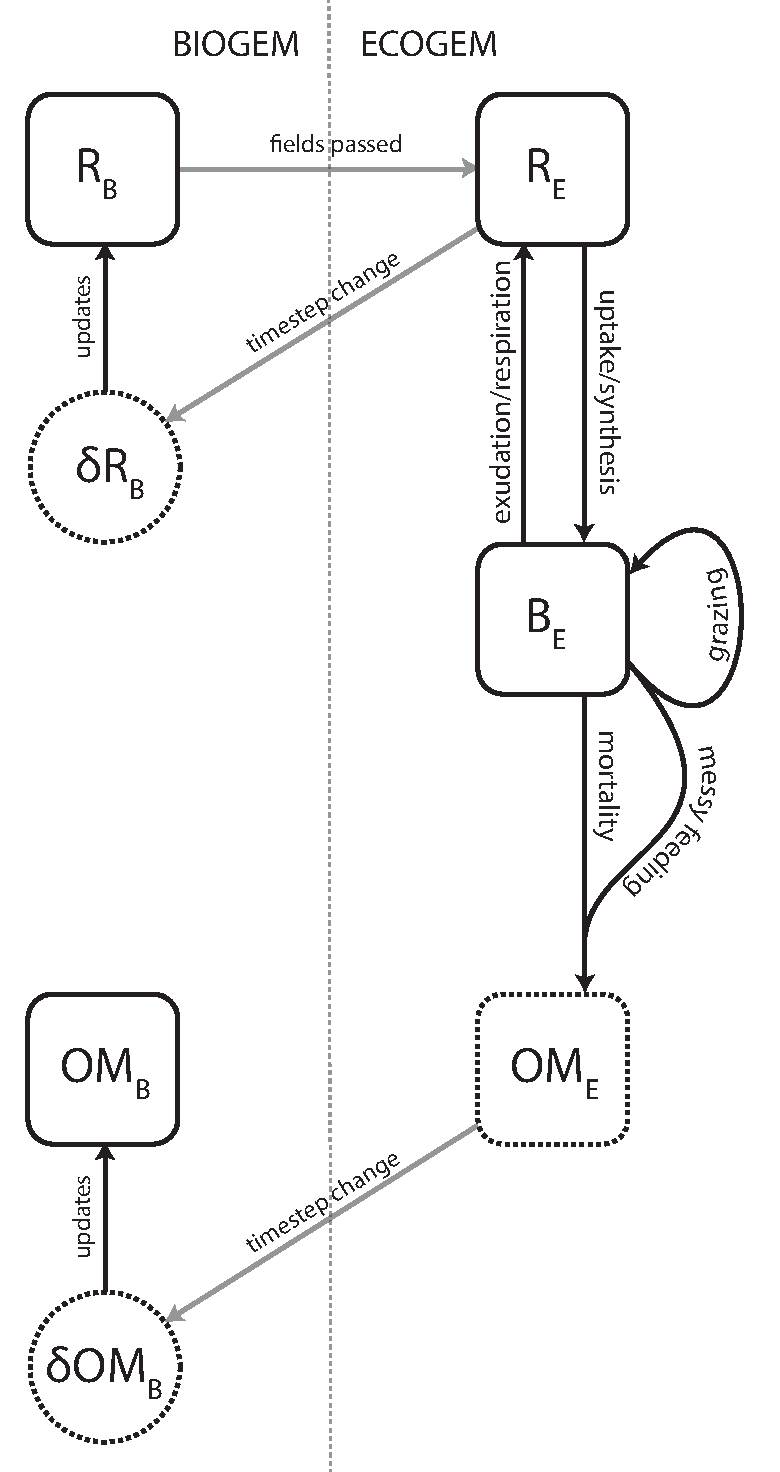
\includegraphics[width=6cm]{Figures/CouplingSchematic.pdf}
\caption{Schematic representation of the coupling between BIOGEM and ECOGEM.}
\label{BIOECOGEM}
\end{figure}

In the following section we outline the key state variables directly relating to ecosystem function (Section~\ref{StateVariables}), describe the mathematical form of the key rate processes relating to each state variable (Section~\ref{PhysiolProc}) and how they link together (Section~\ref{PDEs}). We will then describe the parameterisation of the model according to organism size and functional type (Section~\ref{Parameters}). The model equations are modified from \citet{Ward:2012}. Although we repeat all the equations used in ECOGEM here, we provide only brief descriptions of the parameterisations and parameter values justifications, already included in \citet{Ward:2012}.
 
%-------------------------------------------------------------------------------------------------------------------------------------------------------------------------------------------

\subsection{State variables}\label{StateVariables}

ECOGEM state variables are organised into three matrices (Table~\ref{matrix_table}), representing ecologically-relevant biogeochemical tracers (hereafter referred to as `nutrient resources'), plankton biomass and organic matter. All these matrices have units of mmol element m$^{-3}$, with the exception of the dynamic chlorophyll quota, which is expressed in units of mg~chlorophyll~m$^{-3}$. The nutrient resource matrix ($\matr{R}$) includes $I_r$ distinct inorganic resources. The plankton community ($\matr{B}$) is made up of $J$ individual populations, each associated with $I_b$ cellular nutrient quotas. Finally organic matter ($\matr{D}$) is made up of $K$ size classes of organic matter, each containing $i_d$ organic nutrient element pools. (Note that strictly speaking, biologically dead / detrital organic matter is not explicitly resolved as a state variable in ECOGEM as we currently only resolve the production of organic matter, which is passed to BIOGEM and held there as a state variable.  As a consequence, there is no grazing on detrital organic matter in the current configuration of EcoGENIE. We include  a description of $\matr{D}$ and its relationships here for completeness and for convenience of notation.)

% This matrix formulation allows all plankton populations to be described using the same generic equation. The model structure is therefore highly flexible, and can, in principle, take any number of populations ($J$). The number of nutrient elements and detrital size classes ($I_r$, $I_b$, $I_d$ and $K$) are also flexible, but in practice will be limited to what is also carried available within BIOGEM. 

\begin{table}[htp!]
\begin{center}
\caption{State variable index notation.}
\begin{tabular}{|l|l|c|c|c|}
\hline 
State variable                          & Dimensions                                    &  Index  & Size  &Available elements \\
\hline 
$\matr{R}$                              & Resource element                               &  $i_r$        &  $I_r$        &$\begin{array}{cccccc} DIC, & PO_4, & Fe    \end{array}$ \\
\hline
\multirow{2}{*}{$\matr{B}$}             & Plankton class                                &  $j$    &  $J$          &$\begin{array}{cccc} 1, & 2, & \dots, & $J$    \end{array}$ \\ 
                                                & Cellular quota                                &  $i_b$  &  $I_b$        &$\begin{array}{ccccc} C, & P, & Fe, & Chl      \end{array}$ \\
\hline
\multirow{2}{*}{$\matr{D}$}     & Organic matter size class             &  $k$    &  $K$          &$\begin{array}{cc} DOM, & POM                  \end{array}$ \\
                                                & Detrital nutrient element                     &  $i_d$  &  $I_d$        &$\begin{array}{cccc} C, & P, & Fe                      \end{array}$ \\ 
\hline
\end{tabular} 
\label{matrix_table}
\end{center}
\end{table}



\subsubsection{Inorganic resources}

$\matr{R}$ is a vector of length $I_r$, the number of dissolved inorganic nutrient resources.
%
\begin{equation}
\matr{R}=\left[\begin{array}{cccccc}DIC \\ PO_4 \\ Fe \end{array}\right]
\end{equation}
%
An individual inorganic resource is denoted by the appropriate subscript. For example, $PO_4$ is denoted $R_{PO_4}.$

\subsubsection{Plankton biomass}

$\matr{B}$ is a $I_b\times J$ matrix, where $I_b$ is the number of cellular quotas, including chlorophyll, and $J$ is the number of plankton populations.
%
\begin{equation}
\matr{B}=\left[\begin{array}{cccccc}    B_{C,1} & B_{C,2} & \dots & B_{C,J} \\
                                                        B_{P,1} & B_{P,2} & \dots & B_{P,J} \\
                                                        B_{Fe,1} & B_{Fe,2} & \dots & B_{Fe,J} \\
                                                        B_{Chl,1} & B_{Chl,2} & \dots & B_{Chl,J} \end{array}\right]
\end{equation}
%
Each population and element is denoted by an appropriate subscript. For example, the total carbon biomass of plankton population $j$ is denoted $B_{C,j}$, while the chlorophyll biomass of that population is denoted $B_{Chl,j}$. The vector describing the the carbon content of all plankton populations is denoted $\matr{B}_{C}$.

This framework can account for competition between (in theory) any number of different plankton populations. The model equations (below) are written in terms of an `ideal' planktonic form, with the potential to exhibit the full range of ecophysiological traits (among those that are included in the model). Individual populations may take on a realistic subset of these traits, according to their assigned `plankton functional type' (PFT) (see Section~\ref{community_structure}). Each population is also assigned a characteristic size, in terms of equivalent spherical diameter (ESD) or cell volume. Organism size plays a key role in determining each population's ecophysiological traits (see Section~\ref{size_dep_traits}).

\subsubsection{Organic detritus}

$\matr{D}$ is a $I_d\times K$ matrix, where $I_d$ is the number of detrital nutrient elements, and $K$ is the number of detrital size classes.
%
\begin{equation}
\matr{D}=\left[\begin{array}{cc}        D_{C,1} & D_{C,2}       \\
                                                D_{P,1} & D_{P,2}       \\
                                                D_{Fe,1} & D_{Fe,2}     \end{array}\right]
\end{equation}
%
Each size class and element is denoted by an appropriate subscript. For example, dissolved organic phosphorus (size class $k=1$) is denoted $D_{1,P}$, while particulate organic iron (size class $k=2$) is denoted $D_{2,Fe}$.

%%%%%%%%%%%%%%%%%%%%%%%%%%%%%%%%%%%%%%%%%%%%%%%%%%%%%%%%%%%%%%%%%%%%%%%%%%%%%%

\subsection{Plankton physiology and ecology}\label{PhysiolProc}

The rates of change in each state variable within ECOGEM are defined by a range of ecophysiological processes. These are defined by a set of mathematical functions that are common to all plankton populations. Parameter values are defined in Section~\ref{Parameters}.

%-------------------------------------------------------------------------------------------------------------------------------------------------------------------------------------------

\subsubsection{Temperature limitation}

Temperature affects a wide range of metabolic processes through an Arrenhius-like equation that is here set equal for all plankton.
%
\begin{equation}
\gamma_{\rm T} = e^{A ( {\rm T} - T_{\rm ref} )}
\label{tempfunc}
\end{equation}
%
The parameter $A$ describes the temperature sensitivity, T is the ambient water temperature in degrees C, and $T_{\rm ref}$ is a reference temperature (also in degrees C) at which $\gamma_{\rm T}=1$.

%-------------------------------------------------------------------------------------------------------------------------------------------------------------------------------------------

\subsubsection{The plankton `quota'}

The physiological status of a plankton population is defined in terms of its cellular nutrient quota, $\matr{Q}$, which is the ratio of assimilated nutrient (phosphorus or iron) to carbon biomass. For each plankton population, $j$, and each planktonic quota, $i_b$ ($\ne C$), 
%
\begin{equation}
Q_{i_b,j} = \frac{B_{i_b,j}}{B_{C,j}}
\end{equation}
%
This equation is also used to describe the population chlorophyll content relative to carbon biomass. The size of the quota increases with nutrient uptake, chlorophyll synthesis, or the loss of carbon. The quota decreases through the acquisition of carbon (described below). 

Excessive accumulation of P or Fe biomass in relation to carbon is prevented as the uptake or assimilation of each nutrient element is down-regulated as the respective quota becomes full.  The generic form of the uptake regulation term for element $i_b$ is given by a linear function of the nutrient status, modified by an additional shape-parameter ($h$=$0.1$) that allows greater assimilation under low-to-moderate resource limitation.
%
\begin{equation}
\label{QstatN}
Q_{i_b,j}^{\rm stat}    = \bigg(\frac{Q^{\rm max}_{i_b,j}-Q_{i_b,j}}{Q_{i_b,j}^{\rm max}-Q_{i_b,j}^{\rm min}}\bigg)^h
\end{equation}
%
%-------------------------------------------------------------------------------------------------------------------------------------------------------------------------------------------

\subsubsection{Nutrient uptake}

Phosphate and dissolved iron ($i_r=i_b=$ P or Fe) are taken up as functions of environmental availability ($[R_{i_r}]$), maximum uptake rate ($V_{i_r,j}^{\rm max}$), the nutrient affinity ($\alpha_{i_r,j}$), the quota satiation term, ($Q^{\rm stat}_{i_b,j}$) and temperature limitation ($\gamma_{\rm T}$):
%
\begin{equation}
V_{i_r,j} =   \frac{V_{i_r,j}^{\rm max} \alpha_{i_r,j} {\rm [R_{i_r}]}}{V_{i_r,j}^{\rm max}  + \alpha_{i_r,j}{\rm [R_{i_r}]}} Q^{\rm stat}_{i_b,j} \cdot \gamma_{\rm T}
\end{equation}
%
This equation is effectively equivalent to the Michaelis-Menten type response, but replaces the half-saturation constant with the more mechanistic nutrient affinity, $\alpha_{i_r,j}$.

%\begin{equation}
%V_{i_r,j} = V_{i_r,j}^{\rm max} \frac{{\rm [R_{i_r}]}}{{\rm [R_{i_r}]}+k_{i_r,j}} Q^{\rm stat}_{i_b,j} \cdot \gamma_{\rm T}               
%\end{equation}
%
%-------------------------------------------------------------------------------------------------------------------------------------------------------------------------------------------

\subsubsection{Photosynthesis}

The photosynthesis model is modified from \cite{Geider:1998} and \cite{Moore:2002}. Light-limitation is calculated as a Poisson function of local irradiance ($I$), modified by the iron-dependent initial slope of the P-I curve ($\alpha \gamma_{{\rm Fe},j}$) and the chlorophyll-\textit{a}-to-carbon ratio ($Q_{{\rm Chl},j}$). 
%
\begin{equation}
\label{gammaI}
\gamma_{I,j} = \Big[ 1- \exp \Big( \frac{-\alpha \cdot \gamma_{{\rm Fe},j} Q_{{\rm Chl},j} \cdot { I}}{ P_{{\rm C},j}^{\rm sat}} \Big) \Big]
\end{equation}
%
Here $P_{C,j}^{\rm sat}$ is maximum light-saturated growth rate, modified from an absolute maximum rate of $P_{C,j}^{max}$, according to the current nutrient and temperature limitation terms.
%
\begin{equation}
P_{C,j}^{sat} =  P_{C,j}^{max} \cdot \gamma_T \cdot \min \big[ \gamma_{P,j},~\gamma_{Fe,j} \big]
\end{equation}
%
The nutrient-limitation term is given as a minimum function of the internal nutrient status \citep{Droop:1968,Caperon:1968,Flynn:2008}, each defined by normalised hyperbolic functions for P and Fe ($i_b=$ P or Fe),
%
\begin{equation}
\label{gammaFeP}
\gamma_{i_b,j} =  \frac{1 - Q^{\rm min}_{i_b,j} / Q_{i_b,j} }   {1 - Q^{\rm min}_{i_b,j} / Q^{\rm max}_{i_b,j}  },
\end{equation}
%
The gross photosynthetic rate ($P_{{\rm C},j}$) is then modified from $P_{C,j}^{sat}$ by the light-limitation term.
%
\begin{equation}
P_{{\rm C},j} =   \gamma_{I,j} P_{{\rm C},j}^{\rm sat}
\end{equation}
%
Net carbon uptake, after accounting for the metabolic cost of biosynthesis ($\xi$), is given by 
%
\begin{equation}
V_{{\rm C},j} = P_{{\rm C},j} - \xi \cdot 16V_{{\rm P},j}
\end{equation}
%
This was originally defined as a loss of carbon as a fraction of nitrogen uptake \citep{Geider:1998}. We define it here relative to phosphate uptake, using a fixed N:P ratio of 16.

%-------------------------------------------------------------------------------------------------------------------------------------------------------------------------------------------

\subsubsection{Photoacclimation}

The chlorophyll-to-carbon ratio is regulated as the cell attempts to balance photon capture with the maximum rate at which energy can be used to fix carbon. Depending on this ratio, a certain fraction of newly assimilated nitrogen is diverted to the synthesis of new chlorophyll \textit{a}, 
%
\begin{equation}
\rho_{{\rm Chl},j} = \theta_{\rm N}^{\rm max} \frac{P_{{\rm C},j}}{\alpha \cdot \gamma_{{\rm Fe},j} \cdot Q_{{\rm Chl},j} \cdot {I}}
\end{equation}
%
where $\rho_{{\rm Chl},j}$ is the amount of chlorophyll \textit{a} that is synthesised for every mmol of nitrogen assimilated (mg Chl (mmol N)$^{-1}$). If phosphorus is assimilated at carbon specific rate $V_{{\rm P},j}$ (mmol N (mmol C)$^{-1}$ d$^{-1}$), then the carbon specific rate of chlorophyll \textit{a} synthesis (mg chl (mmol C)$^{-1}$ d$^{-1}$) is
%
\begin{equation}
V_{{\rm Chl},j} = \rho_{{\rm Chl},j} \cdot 16V_{{\rm P},j}
\label{chl_synthesis}
\end{equation}
%
%-------------------------------------------------------------------------------------------------------------------------------------------------------------------------------------------

\subsubsection{Light attenuation}

ECOGEM uses a slightly more complex light attenuation scheme than BIOGEM, which simply calculates a mean solar (shortwave) irradiance averaged over the depth of the mixed layer (by default, equal to the surface layer thickness) and assuming a length scale of 20 m over which light decays [\textcolor{red}{Doney et al., 2006]}. BIOGEM then takes this mean irradiance and applies a Michaelis–Menten like limitation term, assuming a half saturation value for light of 20.0 W m-2 [\textcolor{red}{Doney et al. [2006]}]. At the ocean surface,  the incoming shortwave solar radiation intensity is taken from the climate component in cGENIE and varties seasonally [Edwards and Marsh, 2005; Marsh et al., 2011]. In ECOGEM, productivity is also restricted to the surface layer with the  light level again calculated as the mean level of photosynthetically available radiation within the mixed layer as if the biological population was evenly distributed across the mixed layer \citep[with depth calculated according to][]{Kraus:1967b}. But now we take into account inhibition of light penetration due to the presence of light absorbing molecules and the phenomena of self-shading [\textcolor{red}{REF}].

If $Chl_{tot}$ is the total chlorophyll concentration in the surface layer, $Z_1$ is the thickness of the surface grid box and $Z_{ML}$ is the mixed-layer depth, the  virtual chlorophyll concentration distributed across the mixed layer is given by
%
\begin{equation}
Chl_{ML} = Chl_{tot} \frac{Z_1}{Z_{ML}}
\end{equation}
%
The combined light-attenuation coefficient attributable to both water and the virtual chlorophyll concentration is given by
%
\begin{equation}
 k_{tot}     = k_w + k_{chl}*Chl_{ML}
\end{equation}
%
For a given level of photosynthetically available radiation at the ocean surface ($I_0$), plankton in the surface grid box experience the average irradiance within the mixed layer, which is given by
%
\begin{equation}
I = \frac{I_0}{k_{tot}} \frac{1}{Z_{ML}} (1-e^{(-k_{tot}\cdot Z_{ML})})
\end{equation}
%
%-------------------------------------------------------------------------------------------------------------------------------------------------------------------------------------------

\subsubsection{Predation (including both herbivorous and carnivorous interactions)}

Here we define predation simply as the consumption of any living organism, regardless of the trophic level the organism (i.e. phytoplankton, mixotroph, zooplankton, etc.).

The predator-biomass-specific grazing rate of predator ($j_{\rm pred}$) on prey ($j_{\rm prey}$) is given by,
%
\begin{equation}
G_{{\rm C},j_{\rm pred},j_{\rm prey}} = 
\gamma_{\rm T}
\cdot \underbrace{\frac{G_{{\rm C},j_{\rm pred}}^{\rm max}\alpha_{{\rm C},j_{\rm pred}}\mathcal{F}_{{\rm C},j_{\rm pred}}}{G_{{\rm C},j_{\rm pred}}^{\rm max} + \alpha_{{\rm C},j_{\rm pred}}\mathcal{F}_{{\rm C},j_{\rm pred}} } }_{\rm overall~grazing~rate}
\cdot \underbrace{\Phi_{j_{\rm pred},j_{\rm prey}}}_{\rm switching}
\cdot \underbrace{(1-e^{\Lambda \cdot \mathcal{F}_{{\rm C},j_{\rm pred}}}) }_{\rm prey~refuge}
\label{grazing_func}
\end{equation}
\\
where $\gamma_{\rm T}$ is the temperature-dependence, $G_{{\rm C},j_{\rm pred}}^{\rm max}$ is the maximum grazing rate, and $\alpha_{{\rm C},j_{\rm pred}}$ is the grazing `clearance rate'. The overall grazing rate is a function of total food available to the predator, $\mathcal{F}_{{\rm C},j_{\rm pred}}$. This is given by the product of the prey biomass vector, $\matr{B}_{\rm C}$, and the grazing kernel ($\boldsymbol{\phi}$),
%
\begin{equation}
\boldsymbol{\mathcal{F}}_{\rm C} = \boldsymbol{\phi} \matr{B}_{\rm C}
\end{equation}
%
The grazing kernel is a $J\times J$ matrix describing the relative availability of each prey population to each predator. Each element is an approximately log-normal function of the predator-to-prey length ratio, $\vartheta_{j_{\rm pred},j_{\rm prey}}$, with an optimum ratio of $\vartheta_{\rm opt}$ and a geometric standard deviation $\sigma_{j_{\rm pred}}$. 
%
\begin{equation}
\phi_{j_{\rm pred},j_{\rm prey}} = \exp\Big[-\Big(\ln\big(\frac{\vartheta_{j_{\rm pred},j_{\rm prey}}}{\vartheta_{\rm opt}}\big)\Big)^2  /\big(2\sigma_{j_{\rm pred}}^2\big) \Big]
\end{equation}
%
We also include an optional `prey-switching' term, such that predators may preferentially attack those prey that are relatively more available (i.e. active switching, $s=2$). Alternatively they may attack prey in direct proportion to their availability (i.e. passive switching, $s=1$).
%
\begin{equation}
\Phi_{j_{\rm pred},j_{\rm prey}} = \frac{(\phi_{j_{\rm pred},j_{\rm prey}} {\rm B}_{{\rm C},j_{\rm prey}})^{s}}{\sum_{j_{\rm prey}=1}^J (\phi_{j_{\rm pred},j_{\rm prey}} {\rm B}_{{\rm C},j_{\rm prey}})^{s}}
\label{switching}
\end{equation}
%
Finally, a prey refuge function is incorporated, such that the overall grazing rate is reduced when the availability of all prey ($\mathcal{F}_{{\rm C},j_{\rm pred}}$) is low. The size of the prey refuge is dictated by the coefficient $\Lambda$. The overall grazing response is calculated on the basis of prey carbon. Grazing losses of other prey elements are simply calculated from their stoichiometric ratio to prey carbon, with different elements assimilated according to the predator's nutritional requirements (see below).
%
\begin{equation}
G_{{\rm i_b},j_{\rm pred},j_{\rm prey}} = G_{{\rm C},j_{\rm pred},j_{\rm prey}} \frac{{\rm B}_{i_b,j_{\rm prey}}}{{\rm B}_{{\rm C},j_{\rm prey}}}
\end{equation}
%
%-------------------------------------------------------------------------------------------------------------------------------------------------------------------------------------------

\subsubsection{Prey assimilation} 

Prey biomass is assimilated into predator biomass with an efficiency of $\lambda_{i_b,j_{pred}}$ ($i_b \ne $ Chl). This has a maximum value of $\lambda^{\rm max}$ that is modified according the the quota status of the predator. For elements $i_b$ = P or Fe, prey biomass is assimilated as a function of the respective predator quota. If the quota is full, the element is not assimilated. If the quota is empty, the element is assimilated with maximum efficiency ($\lambda^{\rm max}$). 
%
\begin{equation}
\lambda_{i_b,j_{\rm pred}} = \lambda^{\rm max} Q_{i_b,j}^{\rm stat}
\end{equation}
%
C assimilation is regulated according to the status of the most limiting nutrient element (P or Fe) modified by the same shape-parameter, $h$, that was applied in Equation~\ref{QstatN}. If all three quotas are full, C is assimilated at the maximum rate. If any are empty, C assimilation is down-regulated until sufficient quantities of the limiting element(s) are acquired. 
%
\begin{equation}
Q_{i_b,j}^{\rm lim}     = \bigg( \frac{Q_{i_b,j}-Q^{\rm min}_{i_b,j}}{Q_{i_b,j}^{\rm max}-Q_{i_b,j}^{\rm min}} \bigg)^h
\end{equation}
%
\begin{equation}
\lambda_{C,j_{\rm pred}} = \lambda^{\rm max} \min \big( Q_{P,j}^{\rm lim}, Q_{Fe,j}^{\rm lim}   \big)
\end{equation}
%
%-------------------------------------------------------------------------------------------------------------------------------------------------------------------------------------------

\subsubsection{Respiration}

A linear respiration rate is applied to degrade plankton carbon biomass into dissolved inorganic carbon. This is achieved through a $J$ by $I_r$ respiration matrix, $\matr{r}$, which is non-zero only for $i_r=DIC$.

%-------------------------------------------------------------------------------------------------------------------------------------------------------------------------------------------

\subsubsection{Death}

All living biomass is subject to a linear mortality rate of $m_B$. This rate is reduced at very low biomasses (population carbon biomass $\lesssim$ 1$\times$10${-6}$ mmol C m$^{-3}$) in order to maintain a viable population within every surface grid cell \citep[``everything is everywhere, but the environment selects'',][]{BaasBecking:1934}. 
%
\begin{equation}
m_B = m  (1-e^{-10^{10}\matr{B}_{C}})
\end{equation}
%
The low biomass at which a population attains `immortality' is sufficiently small for that population to have a negligible impact on all other components of the ecosystem.



%%%%%%%%%%%%%%%%%%%%%%%%%%%%%%%%%%%%%%%%%%%%%%%%%%%%%%%%%%%%%%%%%%%%%%







%-------------------------------------------------------------------------------------------------------------------------------------------------------------------------------------------
\subsubsection{Sources of detrital matter}

Plankton mortality and grazing are the only two sources of organic matter, with partitioning between non-sinking dissolved and sinking particulate phases determined by the parameter $\beta_{j}$. 
%
\begin{align}
S^{\rm D}_{i_d,1}       = &     \underbrace{ \sum_{j=1}^{J}  [{\rm B}_{i_d,j}] \beta_{j} m_{\rm P} }_{\rm mortality}                                                   
                                                +       \underbrace{ \sum_{j_{\rm pred}=1}^{J} [{\rm B}_{{\rm C},j_{\rm pred}}] \sum_{j_{\rm prey}=1}^{J} \beta_{j_{\rm prey}} (1-\lambda_{i_b,j_{\rm pred}}) G_{i_d,j_{\rm pred},j_{\rm prey}}}_{\rm messy~feeding}  \\
S^{\rm D}_{i_d,2}       = &     \underbrace{ \sum_{j=1}^{J} [{\rm B}_{i_d,j}] (1-\beta_{j}) m_{\rm P}}_{\rm mortality}                                                         +       \underbrace{ \sum_{j_{\rm pred}=1}^{J} [{\rm B}_{{\rm C},j_{\rm pred}}] \sum_{j_{\rm prey}=1}^{J} (1-\beta_{j_{\rm prey}}) (1-\lambda_{i_b,j_{\rm pred}}) G_{i_d,j_{\rm pred},j_{\rm prey}}}_{\rm messy~feeding}
\end{align}
%
A fixed fraction (66\%) of the organic matter formed in the surface grid-boxes is partitioned directly into dissolved organic matter. This dissolved organic matter is an explicit tracer that is transported by the ocean circulation model and is degraded back to its constituent nutrients with a fixed turnover time of $\lambda$ (= 0.5 years). In this initial implementation of ECOGEM, for traceability, the assumptions are the same as made in the current version of BIOGEM  [\textcolor{red}{REFS}] which themselves follow the OCMIP2 ocean carbon cycle modelling intercomparison protocol described in \textcolor{red}{Najjar et al., 2007}. 

The remaining fraction (34\%) of organic matter is exported vertically from the surface ocean as a flux of particulate organic matter (POM). POM is itself partitioned into two components, a `labile' component which predominantly remineralises in the upper water column, and a `refractory' component that is predominantly remineralised in the deep ocean at the seafloor. The net remineralisation at depth $z$, relative to the export depth $z_{0}$ is determined by characteristic length scales (${l^{\text{POM}}}$ and ${l^{\text{rPOM}}}$ for `labile' and `refractory' POM respectively):
%
\begin{equation} \label{POM_remin}
F_z^{\text{POM}} = F_{z=z_{0}}^{\text{POM}} \cdot  \left( (1-r^{\text{POM}}) \cdot \text{exp}(\frac{z_{0} - z} {l^{\text{POM}}}) \right) + F_{z=z_{0}}^{\text{POM}} \cdot \left( r^{\text{POM}} \cdot \text{exp}(\frac{z_{0} - z} {l^{\text{rPOM}}}) \right) 
\end{equation}
%
The remineralisation length scales reflect a constant sinking speed and constant remineralisation rate. All POM reaching the seafloor is remineralised instantaneously. See \citet{Ridgwell:2007} for a fuller description and justification.

The production and export of calcium carbonate (CaCO$_3$) by calcifying plankton in the surface ocean is scaled to the export of particulate organic carbon via a spatially-uniform scalar which is modified by a thermodynamically-based relationship with the calcite saturation state. The dissolution of CaCO$_3$ below the surface is treated in a similar way to that of particulate organic matter (equation~\ref{POM_remin}), as described by~\citet{Ridgwell:2007} with the parameter values controlling the export ratio between CaCO$_3$ and POC taken from \textcolor{red}{Ridgwell et al. 2007b}.   

%-------------------------------------------------------------------------------------------------------------------------------------------------------------------------------------------
\subsubsection{Oxygen}

Oxygen production is coupled to photosynthetic carbon fixation via a fixed linear ratio, such that 
%
\begin{equation} 
V_{O_2} = -\frac{106}{138} \matr{V}_{DIC} \cdot \matr{B}_C
\end{equation}
%
The negative sign indicates that oxygen is produced as DIC is consumed. Oxygen consumption associated with the remineralisation of organic matter is unchanged relative to BIOGEM.
%-------------------------------------------------------------------------------------------------------------------------------------------------------------------------------------------
\subsubsection{Alkalinity}

Production of alkalinity is coupled to planktonic uptake of PO$_4$ via a fixed linear ratio, such that 
%
\begin{equation} 
V_{Alk} = -16 \matr{V}_{PO_4} \cdot \matr{B}_C
\end{equation}
%
The negative sign indicates that alkalinity increases as PO$_4$ is consumed. This relationship accounts for alkalinity changes associated with N transformations [Zeebe and Wolf-Gladrow, 2001] that are not explicitly represented in this particular biogeochemical configuration of cGENIE (i.e. no N species in the ocean are defined).

%-------------------------------------------------------------------------------------------------------------------------------------------------------------------------------------------
\subsection{Differential equations}\label{PDEs}

Differential equations for ${\matr R}$, ${\matr B}$ and ${\matr D}$ are written out in a generalised matrix form, for application to each element in the state variable matrices. The dimensions of each matrix and vector used equations~\ref{dRdt} to~\ref{dDdt} are given in Table~\ref{matrix_table}. In the following equations the `$\cdot$' symbol denotes a dot product operation, while `$\circ$' denotes entrywise multiplication (the Hadamard product).

Note that while $\matr{R}$ and $\matr{OM}$ are transported by the physical component of GENIE, living biomass $\matr{B}$ is not currently subject to any physical transport. The only communication between biological communities in adjacent grid cells is through the advection and diffusion of inorganic resources and non-living organic matter in BIOGEM. Note that some additional sources and sinks of $\matr{R}$, and all sinks of $\matr{D}$, are computed in BIOGEM.

\subsubsection{Inorganic resources}

For each inorganic resource, $i_r$, 
%
\begin{align}
\frac{\partial {R_{i_r}}}{\partial t}   =       &- \underbrace{\matr{V}_{i_r} \cdot \matr{B}_C}_{\rm uptake}
                                                                     + \underbrace{\matr{r}_{i_r} \cdot \matr{B}_C}_{\rm respiration}  \label{dRdt}
\end{align}
%

\subsubsection{Plankton biomass}

For each plankton class, $j$, and internal biomass quota, $i_b$,
%
\begin{align}
\frac{\partial B_{i_b,j}}{\partial t}   =       &+ \underbrace{V_{i_b,j} B_{C,j}}_{\rm uptake}    
                                                                   - \underbrace{m_{j} B_{i_b,j}}_{\rm basal~mortality}                %\nonumber\\
                                                                 + \underbrace{B_{C,j}  (\boldsymbol{\lambda}_{i_b} \cdot \matr{G}_{i_b}^{\rm gain})   }_{\rm grazing~gains}         
                                                                    - \underbrace{r_{i_b,j} B_{C,j}}_{\rm respiration}
                                                                    - \underbrace{\matr{B}_C \cdot \matr{G}_{i_b}^{\rm loss}         }_{\rm grazing~losses}          \label{dBdt}
\end{align}
%
\subsubsection{Organic detritus}

For each detrital nutrient element, $i_d$, and detritral size class, $k$
%
\begin{align}
\frac{\partial {\rm D}_{i_d,k}}{\partial t}     =       &       + \underbrace{  \Big[\boldsymbol{\beta}_{k} \circ (1-\boldsymbol{\lambda}_{i_b})\Big] \matr{G}_{i_b} \matr{B}_C}_{\rm unassimilated~grazing}          + \underbrace{  \Big[\boldsymbol{\beta}_{k} \circ \matr{m}\Big] \matr{B}_{i_b} }_{\rm other~mortality}      \label{dDdt}
\end{align}
%
The relative fraction of detrital matter passed to DOM is given by the parameter $\beta$, which is here assigned a constant value of 0.66 for all populations \citep{Ridgwell:2007}.

\subsubsection{Coupling to BIOGEM}

The calculations in BIOGEM are performed once for every 2 time-steps taken by the ocean circulation model (i.e. 48 time-steps per year). [\textcolor[rgb]{0.501961,0,1}{ECOGEM\ TIMESTEP???}]
Each ECOGEM time-step, concentrations of inorganic tracers and key properties of the physical environment are passed from BIOGEM, and the ecological community responds by transforming inorganic compounds into living biomass through photosynthesis.  At the end of each ECOGEM time step, the rates of change in $\bf{R}$ and $\bf{OM}$ are passed back to BIOGEM. ${\partial {\matr R}}/{\partial t}$ is used to update DIC, phosphate and iron tracers, while ${\partial {\matr D}_{DOM}}/{\partial t}$ is added to the dissolved organic matter pools. The rate of particulate organic matter production, ${\partial {\matr D}_{POM}}/{\partial t}$ is instantly remineralised at depth using to the standard BIOGEM export functions. $\frac{\partial {\matr B}}{\partial t}$ is used only to update the living biomass concentrations within ECOGEM. The structure of the coupling is illustrated in Figure~\ref{BIOECOGEM}.





In the initial implementation of ECOGEM described and evaluated here, the explicit plankton community is held entirely within the ECOGEM module and is not subject to physical transport (e.g. advection and diffusion) the  ocean circulation model (although dissolved tracers such as nutrients still are). [\textcolor[rgb]{0.501961,0,1}{ADD\ BRIEF\ JUSTIFICATION\ AS\ TO\ WHY\ WE\ THINK\ THIS\ IS\ OK TO\ A\ FIRST\ APPROX}] 
On-line advection of ecosystem state variables will be implemented and its consequences explored in a future version of EcoGENIE. 

%-------------------------------------------------------------------------------------------------------------------------------------------------------------------------------------------
\subsection{Ecophysiological parameterisation}\label{Parameters}

The model community is made up of a number of different plankton populations, with each one described according to the same set of equations, as outlined above. Differences between the populations are specified according to individual parameterisation of those equations. In the following sections, we describe how the members of the plankton community are specified for evaluation, and how their parameters are assigned according to the organism's size and taxonomic group.

\subsubsection{Model structure}\label{community_structure}

The plankton community in ECOGEM is designed to be highly configurable. Each population present in the initial community is specified by a single line in an input text file, which describes the organism size and taxonomic group.


In this configuration we include 16 plankton populations across eight different size classes. These are divided into two PFTs, namely, ``Phytoplankton'' and `Zooplankton'' (see Table~\ref{planktonconfig}). The eight phytoplankton populations have nutrient uptake and photosynthesis traits enabled, and predation traits disabled, whereas the opposite is true for the eight zooplankton populations. In future we expect to bring in a wider range of trait-based functional types, including siliceous plankton \citep[e.g.][]{Follows:2007}, calcifiers \citep{Monteiro:2016}, nitrogen fixers \citep{Monteiro:2010}, and mixotrophs \citep{Ward:2016}.

\begin{table}[htp!]
\begin{center}
\caption{Plankton functional groups and sizes in the standard run.}
\begin{tabular}{rlS[table-format=3.2]}
\hline
$j$     & PFT                   & \multicolumn{1}{r}{ESD ($\mu$m)}  \\
\hline
1       & Phytoplankton         & 0.6  \\
2       & Phytoplankton         & 1.9  \\
3       & Phytoplankton         & 6.0  \\
4       & Phytoplankton         & 19.  \\
5       & Phytoplankton         & 60.  \\
6       & Phytoplankton         & 190.  \\
7       & Phytoplankton         & 600.  \\
8       & Phytoplankton         & 1900.  \\
\hline 
\end{tabular} 
\begin{tabular}{rlS[table-format=3.2]}
\hline
$j$     & Functional Type       & \multicolumn{1}{r}{ESD ($\mu$m)}  \\
\hline
11      & Zooplankton           & 0.6  \\
12      & Zooplankton           & 1.9  \\
13      & Zooplankton           & 6.0  \\
14      & Zooplankton           & 19.  \\
15      & Zooplankton           & 60.  \\
16      & Zooplankton           & 190.  \\
17      & Zooplankton           & 600.  \\
18      & Zooplankton           & 1900.  \\
\hline 
\end{tabular} 
\label{planktonconfig}
\end{center}
\end{table}

\subsubsection{Size-dependent traits}\label{size_dep_traits}

The size-dependent ecophysiological parameters ($p$) given in Table~\ref{Size_dependent} are assigned as a function of organismal volume ($V=\pi [ESD]^3/6$) according to standard allometric relationships of the form,
%
\begin{equation}
p=a\Big(\frac{V}{V_0}\Big)^b
\end{equation}
%
Here $V_0$ is a reference value of $V_0$ = 1 $\mu$m$^3$. The value of $p$ at $V=V_0$ is given by the coefficient $a$, while the rate of change in $p$ as a function of $V$ is described by the exponent $b$.

\begin{table*}[htp!]
\footnotesize
\caption{Size-dependent ecophysiological parameters ($p$) and power-law parameters ($a$ and $b$), such that ${p=a\Big(\frac{V}{V_0}\Big)^b}$.}
\begin{tabular*}{1.0\textwidth}{@{\extracolsep{\fill}}llllll}
\hline \\ [-2ex]
\multicolumn{2}{l}{Parameter}                           & Symbol                                                & \multicolumn{2}{l}{Power-law parameters}                & Units                                                  \\ 
&                                                                       & $p$                                             & $a$                           & $b$             &                                                       \\ 
\multicolumn{5}{l}{{Inorganic nutrient uptake}}\\ 
%&Maximum uptake rate                                   & $V^{\rm max}_{\rm NO_3}$          & 0.44                          & -0.12         & mmol N (mmol C)$^{-1}$ d$^{-1}$        \\ 
%&                                                                      & $V^{\rm max}_{\rm NO_2}$                & 0.44                          & -0.12           & mmol N (mmol C)$^{-1}$ d$^{-1}$       \\ 
%&                                                                      & $V^{\rm max}_{\rm NH_4}$                & 0.22                          & -0.12           & mmol N (mmol C)$^{-1}$ d$^{-1}$       \\ 
&Maximum uptake rates                                   & $V^{\rm max}_{\rm PO_4}$          & 4.4$\times10^{-2}$            & 0.06          & mmol P (mmol C)$^{-1}$ d$^{-1}$        \\ 
&                                                                       & $V^{\rm max}_{\rm Fe}$                  & 1.4$\times10^{-5}$            & -0.09           & mmol Fe (mmol C)$^{-1}$ d$^{-1}$      \\ 
%&Half-saturation concentration                         & $k_{\rm NO_3}$                                & 0.14                            & 0.33          & mmol N m$^{-3}$                               \\ 
%&                                                                      & $k_{\rm NO_2}$                          & 0.14                          & 0.33            & mmol N m$^{-3}$                               \\ 
%&                                                                      & $k_{\rm NH_4}$                          & 0.07                          & 0.33            & mmol N m$^{-3}$                               \\ 
&Half-saturation concentrations                         & $k_{\rm PO_4}$                                & 0.04                            & 0.41          & mmol P m$^{-3}$                               \\ 
&                                                                       & $k_{\rm Fe}$                                    & 8.0$\times10^{-6}$            & 0.27            & mmol Fe m$^{-3}$                              \\ 
\multicolumn{6}{l}{{Carbon quotas}}             \\ 
&Cell carbon content                                    & $Q_{\rm C}$                                   & 1.45$\times10^{-11}$    & 0.88          & mmol C cell$^{-1}$                            \\ 
\multicolumn{6}{l}{{Grazing}}\\
&Maximum prey ingestion rate                            & $G^{max}_{\rm C}$                     & 21.9                            & -0.16         & d$^{-1}$                                              \\ 
\hline\\  [-1ex]
\end{tabular*}
\label{Size_dependent}
\end{table*}

%limited to values between 0 and 1. It is here assumed to be given by a sigmoidal function of organism ESD, according to three adjustable parameters ($\beta_a$, $\beta_b$, and $\beta_c$) as outlined in Table~\ref{tab:beta}. 

%\begin{equation}
%\beta_j        = \beta_a - \frac{\beta_a - \beta_b}{1+\beta_c/{\rm ESD}_j}
%\end{equation}
%

%\begin{table*}[htp!]
%\footnotesize
%\caption{Parameters describing the size-dependent partitioning of detrital material between the dissolved and (implicit) particulate pools.}
%\begin{tabular*}{1.0\textwidth}{@{\extracolsep{\fill}}lllll}
%\hline \\ [-2ex]
%Parameter              & Meaning                                                                       & $\beta_{mort}$  & $\beta_{graz}$        & Units                         \\
%$\beta_a$              & Maximum fraction to DOM as $ESD\rightarrow0$          & 1.0                             & 1.0                           & dimensionless \\
%$\beta_b$              & Minimum fraction to DOM as $ESD\rightarrow\infty$     & 0.7                             & 0.7                           & dimensionless \\
%$\beta_c$              & Reference diameter at which $\beta=0.5$                       & 10                              & 100                   & $\mu$m                        \\
%\hline\\  [-1ex]
%\end{tabular*}
%\label{tab:beta}
%\end{table*}

%\begin{figure}[htbp]
%\begin{center}
%\includegraphics[width=9cm]{Figures/OM_fractionation.png}
%\caption{Size-dependent fraction of mortality and unassimilated feeding pased to DOM ($\beta$). Dots indicate size classes used in the model.}
%\label{fig:OMfraction}
%\end{center}
%\end{figure}

\subsubsection{Size-independent traits}\label{size_ind_traits}

A list of size-independent model parameters are listed in Table~\ref{Size_independent}.

\begin{table*}[htp!]
\footnotesize
\caption{Size-independent model parameters.}
\begin{tabular*}{1.0\textwidth}{@{\extracolsep{\fill}}lllll}
\hline \\ [-2ex]
\multicolumn{2}{l}{{Parameter}}                         &{Symbol}                               & {Value}                         & {Units}       \\  [+2ex]
%\multicolumn{5}{l}{{Nutrient uptake}} \\  
%& Ammonium inhibition                                  & $\Psi$                                        & 4.6                                     & (mmol N m$^{-3})^{-1}$        \\  
\multicolumn{5}{l}{{Nutrient quotas}} \\  
%& Minimum nitrogen:carbon quota                        & $Q^{\rm min}_{\rm N}$             & 5.0$\times10^{-2}$            & mmol N (mmol C)$^{-1}$        \\  
%& Maximum nitrogen:carbon quota                        & $Q^{\rm max}_{\rm N}$             & 1.7$\times10^{-1}$            & mmol N (mmol C)$^{-1}$        \\ 
& Minimum phosphate:carbon quota                        & $Q^{\rm min}_{\rm P}$             & 2.1$\times10^{-3}$            & mmol P (mmol C)$^{-1}$        \\  
& Maximum phosphate:carbon quota                        & $Q^{\rm max}_{\rm P}$             & 1.1$\times10^{-2}$            & mmol P (mmol C)$^{-1}$        \\   
& Minimum iron:carbon quota                             & $Q^{\rm min}_{\rm Fe}$            & 1.0$\times10^{-6}$            & mmol Fe (mmol C)$^{-1}$       \\  
& Maximum iron:carbon quota                             & $Q^{\rm max}_{\rm Fe}$    & 4.0$\times10^{-6}$            & mmol Fe (mmol C)$^{-1}$       \\  
\multicolumn{5}{l}{{Temperature}}               \\  
& Reference temperature                                 & $T_{\rm ref}$                         & 20                                      & $^\circ$C     \\  
& Temperature dependence                                & $A$                                   & 0.05                            & -                     \\  
\multicolumn{5}{l}{{Photosynthesis}}    \\  
& Maximum Chl-\textit{a}-to-nitrogen ratio              & $\theta^{\rm max}_{\rm N}$     & 3.0                                   & mg Chl \textit{a} (mmol N)$^{-1}$       \\  
& Initial slope of P-I curve                                    & $\alpha$                              & 3.83$\times10^{-7}$     & mmol C (mg Chl \textit{a})$^{-1}$($\mu$Ein m$^{-2}$)$^{-1}$         \\  
& Cost of biosynthesis                                  & $\xi$                                 & 2.33                            & mmol C (mmol N)$^{-1}$        \\ 
\multicolumn{5}{l}{{Grazing}}\\  
& Optimum predator:prey length ratio            & $\vartheta_{\rm opt}$         & 10                                      & -     \\  
& Geometric s.d. of $\vartheta$                         & $\sigma_{\rm graz}$           & 2.0                                     & -     \\  
& Total prey half-saturation                            & $k^{\rm prey}_{\rm C}$             & 5.0                                   & mmol C m$^{-3}$       \\  
& Maximum assimilation efficiency                       & $\lambda^{\rm max}$           & 0.7                                     & -     \\  
& Grazing refuge parameter                              & $\Lambda$                             & -1                                      & (mmol C m$^{-3}$)$^{-1}$      \\  
& Assimilation shape parameter                  & $h$                                   & 0.1                                     & -     \\  
\multicolumn{5}{l}{{Other loss terms}}\\  
& Plankton mortality                                            & $m$                                   & 0.05                            & d$^{-1}$      \\  
& Plankton respiration                                  & $r_{DIC}$                             & 0.05                            & d$^{-1}$      \\  
\multicolumn{4}{l}{{Light attenuation}}         \\  
&Light attenuation by water                             & $k_{\rm w}$                           & 0.04                            & m$^{-1}$                                      \\  
&Light attenuation by chlorophyll                       & $k_{\rm Chl}$                         & 0.03                            & m$^{-1}$(mg Chl)$^{-1}$               \\  [+1ex]
\hline\\  [-1ex]
\end{tabular*}
\label{Size_independent}
\end{table*}


\subsection{Parameter modifications}

As far as possible, the parameter values applied in  ECOGEM were kept as close as possible to previously published versions of the model \citep{Ward:2016}. There were however a few modifications that were required to bring EcoGENIE into first order agreement with observations and the current version  of cGENIE \citep{Ridgwell:prep}. In particular, in comparison to the biogeochemical model used in \citet{Ward:2016}, the amount of soluble iron supplied to cGENIE by atmospheric deposition is considerably less. With a smaller source of iron, it was necessary to reduce the iron demand of the plankton community, and this was achieved by reducing $Q^{\rm max}_{\rm Fe}$ and $Q^{\rm min}_{\rm Fe}$ by five-fold ($Q^{\rm max}_{\rm Fe}$ from 20 to 4 nmol Fe (mmol C)$^{-1}$, and $Q^{\rm min}_{\rm Fe}$ from 5 to 1 nmol Fe (mmol C)$^{-1}$).

We also found that the flexible stoichiometry of ECOGEM led to excessive export of carbon from the surface ocean, attributable to higher C:P ratios in organic matter (BIOGEM assumes a Redfieldian C:P of 106). This effect was moderated by adding the respiration term, which returns a fraction of carbon biomass directly to DIC (it is assumed that other elements are not lost in this way). The additional production of POC also led to increased production of calcium carbonate. This was counteracted by reducing the PIC:POC production ratio from \textbf{[\textcolor{red}{X to Y}]}.

%%%%%%%%%%%%%%%%%%%%%%%%%%%%%%%%%%%%%%%%%%%%%%%%%%%%%%%%%%%%%%%%%%%%%%%
\section{Simulations and Data}\label{SimData}

\subsection{10,000 year spin-up}

We ran cGENIE (as configured and described in \citep{Ridgwell:prep}) and EcoGENIE (as described here) each for period of 10,000 years. These runs were initialised from a homogenous and static ocean, with an imposed constant atmospheric CO$_2$ concentration of 278 ppm. We present model output from the 10,000th year of integration. 

\subsection{Observations}

 Although they are not necessarily strictly comparable (discussed later), we compare results from the pre-industrial configurations of cGENIE and EcoGENIE to contemporary climatologies from a range of sources. Global climatologies of dissolved phosphate and oxygen are drawn from the World Ocean Atlas (WOA 2009), while DIC and alkalinity are taken from Global Ocean Data Analysis Project (GLODAP). Surface chlorophyll concentrations represent a climatological average from 1997 to 2002, estimated by the SeaWiFS satellite.  Depth-integrated primary production is from \citet{Behrenfeld:1997}. All of these interpolated global fields have been re-gridded onto the cGENIE 36\(\times\)36\(\times\)16 grid.

Observed dissolved iron concentrations are those published by Tagliabue et al. (2012). These data are too sparse and variable to allow reliable mapping on the cGENIE grid, and are therefore shown as individual data.

Fidelity to the observed seasonal cycle of nutrients and biomass was evaluated against observations from nine Joint Global Ocean Flux Study (JGOFS) sites: the Hawai`i Ocean Time-series (HOT: 23$^\circ$N, 158$^\circ$W), the Bermuda Atlantic Time-series Study (BATS: 32$^\circ$N, 64$^\circ$W), the equatorial Pacific (EQPAC: 0$^\circ$N, 140$^\circ$W), the Arabian Sea (ARABIAN: 16$^\circ$N, 62$^\circ$E), the North Atlantic Bloom Experiment (NABE: 47$^\circ$N, 19$^\circ$W), station P (STNP: 50$^\circ$NS, 145$^\circ$W), Kerfix (KERFIX: 51$^\circ$S, 68$^\circ$E), Antarctic Polar Frontal Zone (APFZ: 62$^\circ$S, 170$^\circ$W) and the Ross Sea (ROSS: 75$^\circ$S, 180$^\circ$W). Model output for KERFIX and the Ross Sea site was not taken at the true locations of the observations (51$^\circ$S, 68$^\circ$E and 75$^\circ$S, 180$^\circ$W, respectively). Kerfix was moved to compensate for a poor representation of the Polar Front within the coarse resolution ocean model, while the Ross Sea site does not lie within the GEnIE ocean grid. At each site, the observational data represent the mean daily value within the mixed layer. Data from all years are plotted together as one climatological year.

% global surface BGC
\section{Results}\label{Results}

\subsection{Biogeochemical variables}

We start by describing the global distributions of key biogeochemical tracers that are common to both cGENIE and EcoGENIE.

\subsubsection{Global surface values}

Annual mean global distributions are presented for the upper 80.8~m of the water column, corresponding to the model surface layer. In Figure~\ref{fig:nutrients} we compare output from the two models to observations of dissolved phosphate and iron. Surface phosphate concentrations are broadly similar between the two versions of the model, except that EcoGENIE slightly underestimates concentrations in the Southern Ocean. Both versions strongly underestimate surface phosphate in the equatorial and north Pacific, and to a lesser extent in the north and east Atlantic, the Arctic and the Arabian Sea. This is likely attributable in part to the model underestimating the strength of upwelling in these regions. It should also be noted that the observations may in some cases be unrepresentative of the true surface layer, when this is significantly less than 80.8 m. In such cases the observed value will be affected by measurements from below the surface layer. Iron distributions are also broadly similar between the two models, with EcoGENIE showing slightly lower iron concentrations over most of the ocean. 

Figure~\ref{fig:carbon} shows observed and modelled values of inorganic carbon, alkalinity and oxygen. The two models yield very similar surface distributions of the three tracers. DIC and alkalinity are both broadly underestimated relative to observations, while oxygen shows higher fidelity, albeit with artificially high estimates in the equatorial Pacific. This is likely attributable to artificially weak upwelling in this region. 

Surface $\Delta$pCO$_2$ from the two models is shown in Figure~\ref{fig:dpCO2}. EcoGENIE shows weaker CO$_2$ outgassing in tropical band, with a much stronger ocean-to-atmosphere flux in the Western Arctic. 

In Figure~\ref{fig:particulates} we show the annual mean rate of particulate organic matter production in the surface layer. In comparison to cGENIE, EcoGENIE shows elevated POC production in all regions. \textbf{[NEED TO PLOT RATIOS of ECOGEM:BIOGEM, as differences will probably be clearer...]}. Production of CaCO$_3$ is globally less variable in EcoGENIE than cGENIE, with notable higher fluxes in the oligotrophic gyres and polar regions. 

The relative proportions in which these elements and compounds are exported from the surface ocean are regulated by the stoichiometry of biological production. In BIOGEM, carbon and phosphorus production are rigidly coupled through a fixed ratio of 106:1, while POFe:POC and CaCO$_3$:POC production ratios are regulated as a function of environmental conditions. In ECOGEM, phosphorus, iron and carbon production are all decoupled through the flexible quota physiology, which depends on both environmental conditions, and the status of the food-web. Only CaCO$_3$:POC production ratios are regulated via the same mechanism in the two models (although we reduced the average CaCO$_3$:POC ratio in ECOGEM to compensate for the elevated POC production relative to POP). 

\begin{figure}[htp]
\begin{subfigure}{.33\textwidth}
  \centering
  \caption{PO$_4$ - WOA (2009)}
  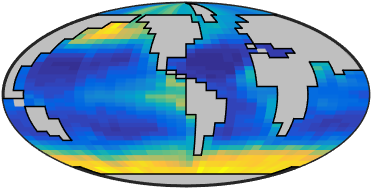
\includegraphics[width=0.95\linewidth]{/Users/ward/cgenie_output/WOA_2009_data/surface_p_an.png}
  \label{fig:nutrients1}
\end{subfigure}%
\begin{subfigure}{.33\textwidth}
  \centering
  \caption{PO$_4$ - BIOGEM}
  \includegraphics[width=0.95\linewidth]{/Users/ward/cgenie_output/BENW.worjh2.PO4FeTDTL_HYBRID_new.SPIN/figures/ocn_PO4.png}
  \label{fig:nutrients1}
\end{subfigure}%
\begin{subfigure}{.33\textwidth}
  \centering
  \caption{PO$_4$ - ECOGEM}
  \includegraphics[width=0.95\linewidth]{/Users/ward/cgenie_output/BENW.worjh2.PO4FeTDTL_HYBRID_WF16_tgld_new.SPIN/figures/ocn_PO4.png}
  \label{fig:nutrients2}
\end{subfigure}
\\[+0.2cm]
\begin{subfigure}{.5\textwidth}
  \centering
  
\includegraphics[width=0.95\linewidth]{/Users/ward/cgenie_output/BENW.worjh2.PO4FeTDTL_HYBRID_WF16_tgld_new.SPIN/figures/ocn_PO4_clrbr.png}
\end{subfigure}
\begin{subfigure}{.33\textwidth}
  \centering
  \caption{dFe - \citet{Tagliabue:2012}}
  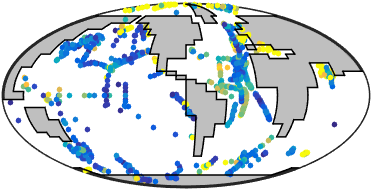
\includegraphics[width=0.95\linewidth]{/Users/ward/cgenie_output/Tagliabue_data/surface_fe.png}
  \label{fig:nutrients1}
\end{subfigure}%
\begin{subfigure}{.33\textwidth}
  \centering
  \caption{dFe - BIOGEM}
  \includegraphics[width=0.95\linewidth]{/Users/ward/cgenie_output/BENW.worjh2.PO4FeTDTL_HYBRID_new.SPIN/figures/ocn_TDFe.png}
  \label{fig:nutrients3}
\end{subfigure}%
\begin{subfigure}{.33\textwidth}
  \centering
  \caption{dFe - ECOGEM}
  \includegraphics[width=0.95\linewidth]{/Users/ward/cgenie_output/BENW.worjh2.PO4FeTDTL_HYBRID_WF16_tgld_new.SPIN/figures/ocn_TDFe.png}
  \label{fig:nutrients4}
\end{subfigure}
\\[+0.2cm]
\begin{subfigure}{.5\textwidth}
  \centering
  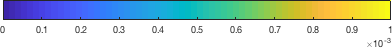
\includegraphics[width=0.95\linewidth]{/Users/ward/cgenie_output/BENW.worjh2.PO4FeTDTL_HYBRID_WF16_tgld_new.SPIN/figures/ocn_TDFe_clrbr.png}
\end{subfigure}
\caption{Surface concentrations of dissolved inorganic nutrients.}
\label{fig:nutrients}
\end{figure}

\begin{figure}[htp]
\begin{subfigure}{.33\textwidth}
  \centering
  \caption{DIC - GLODAP}
  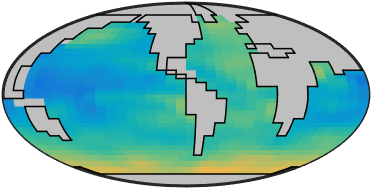
\includegraphics[width=0.95\linewidth]{/Users/ward/cgenie_output/GLODAP_data/surface_TCO2.png}
  \label{fig:nutrients1}
\end{subfigure}%
\begin{subfigure}{.33\textwidth}
  \centering
  \caption{DIC - BIOGEM}
  \includegraphics[width=0.95\linewidth]{/Users/ward/cgenie_output/BENW.worjh2.PO4FeTDTL_HYBRID_new.SPIN/figures/ocn_DIC.png}
  \label{fig:carbon1}
\end{subfigure}%
\begin{subfigure}{.33\textwidth}
  \centering
  \caption{DIC - ECOGEM}
  \includegraphics[width=0.95\linewidth]{/Users/ward/cgenie_output/BENW.worjh2.PO4FeTDTL_HYBRID_WF16_tgld_new.SPIN/figures/ocn_DIC.png}
  \label{fig:carbon2}
\end{subfigure}
\\[+0.2cm]
\begin{subfigure}{.5\textwidth}
  \centering
  
\includegraphics[width=0.95\linewidth]{/Users/ward/cgenie_output/BENW.worjh2.PO4FeTDTL_HYBRID_WF16_tgld_new.SPIN/figures/ocn_DIC_clrbr.png}
\end{subfigure}
\begin{subfigure}{.33\textwidth}
  \centering
  \caption{Alkalinity - GLODAP}
  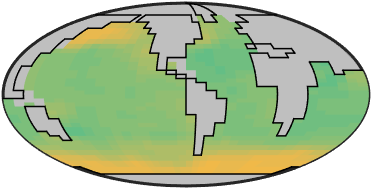
\includegraphics[width=0.95\linewidth]{/Users/ward/cgenie_output/GLODAP_data/surface_PALK.png}
  \label{fig:nutrients1}
\end{subfigure}%
\begin{subfigure}{.33\textwidth}
  \centering
  \caption{Alkalinity - BIOGEM}
  \includegraphics[width=0.95\linewidth]{/Users/ward/cgenie_output/BENW.worjh2.PO4FeTDTL_HYBRID_new.SPIN/figures/ocn_ALK.png}
  \label{fig:carbon3}
\end{subfigure}%
\begin{subfigure}{.33\textwidth}
  \centering
  \caption{Alkalinity - ECOGEM}
  \includegraphics[width=0.95\linewidth]{/Users/ward/cgenie_output/BENW.worjh2.PO4FeTDTL_HYBRID_WF16_tgld_new.SPIN/figures/ocn_ALK.png}
  \label{fig:carbon4}
\end{subfigure}
\\[+0.2cm]
\begin{subfigure}{.5\textwidth}
  \centering
  
\includegraphics[width=0.95\linewidth]{/Users/ward/cgenie_output/BENW.worjh2.PO4FeTDTL_HYBRID_WF16_tgld_new.SPIN/figures/ocn_ALK_clrbr.png}
\end{subfigure}
\begin{subfigure}{.33\textwidth}
  \centering
  \caption{Oxygen - WOA (2009)}
  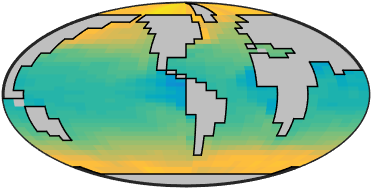
\includegraphics[width=0.95\linewidth]{/Users/ward/cgenie_output/WOA_2009_data/surface_o_an.png}
  \label{fig:nutrients1}
\end{subfigure}%
\begin{subfigure}{.33\textwidth}
  \centering
  \caption{Oxygen - BIOGEM}
  \includegraphics[width=0.95\linewidth]{/Users/ward/cgenie_output/BENW.worjh2.PO4FeTDTL_HYBRID_new.SPIN/figures/ocn_O2.png}
  \label{fig:carbon3}
\end{subfigure}%
\begin{subfigure}{.33\textwidth}
  \centering
  \caption{Oxygen - ECOGEM}
  \includegraphics[width=0.95\linewidth]{/Users/ward/cgenie_output/BENW.worjh2.PO4FeTDTL_HYBRID_WF16_tgld_new.SPIN/figures/ocn_O2.png}
  \label{fig:carbon4}
\end{subfigure}
\\[+0.2cm]
\begin{subfigure}{.5\textwidth}
  \centering
  
\includegraphics[width=0.95\linewidth]{/Users/ward/cgenie_output/BENW.worjh2.PO4FeTDTL_HYBRID_WF16_tgld_new.SPIN/figures/ocn_O2_clrbr.png}
\end{subfigure}
\caption{Surface concentrations of dissolved inorganic carbon, alkalinity and dissolved oxygen.}
\label{fig:carbon}
\end{figure}


\begin{figure}[htp]
\begin{subfigure}{.33\textwidth}
  \centering
  \caption{$\Delta$pCO$_2$ (ppm) - BIOGEM}
  \includegraphics[width=0.95\linewidth]{/Users/ward/cgenie_output/BENW.worjh2.PO4FeTDTL_HYBRID_new.SPIN/figures/atm_dpCO2.png}
  \label{fig:dpCO2_1}
\end{subfigure}%
\begin{subfigure}{.33\textwidth}
  \centering
  \caption{$\Delta$pCO$_2$ (ppm) - ECOGEM}
  \includegraphics[width=0.95\linewidth]{/Users/ward/cgenie_output/BENW.worjh2.PO4FeTDTL_HYBRID_WF16_tgld_new.SPIN/figures/atm_dpCO2.png}
  \label{fig:dpCO2_2}
\end{subfigure}
\\[+0.2cm]
\begin{subfigure}{.5\textwidth}
  \centering
  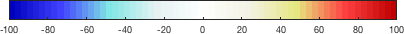
\includegraphics[width=0.95\linewidth]{/Users/ward/cgenie_output/BENW.worjh2.PO4FeTDTL_HYBRID_WF16_tgld_new.SPIN/figures/atm_dpCO2_clrbr.png}
\end{subfigure}
\caption{(Preindustrial) surface $\Delta$pCO$_2$.}
\label{fig:dpCO2}
\end{figure}




\begin{figure}[htp]
%%%%%%%%%%%%%%%%%%%%%%%%%%%%%%%%%%%%%%%%%%%%%%%%%%%%%%%%%%%%
\begin{subfigure}{.33\textwidth}
  \centering
  \caption{POC production - BIOGEM}
  \includegraphics[width=0.95\linewidth]{/Users/ward/cgenie_output/BENW.worjh2.PO4FeTDTL_HYBRID_new.SPIN/figures/bio_fpart_POC.png}
  \label{fig:dpCO2_1}
\end{subfigure}%
\begin{subfigure}{.33\textwidth}
  \centering
  \caption{POC production - ECOGEM}
  \includegraphics[width=0.95\linewidth]{/Users/ward/cgenie_output/BENW.worjh2.PO4FeTDTL_HYBRID_WF16_tgld_new.SPIN/figures/bio_fpart_POC.png}
  \label{fig:dpCO2_2}
\end{subfigure}
\begin{subfigure}{.33\textwidth}
  \centering
  \caption{ECOGEM$\div$BIOGEM}
  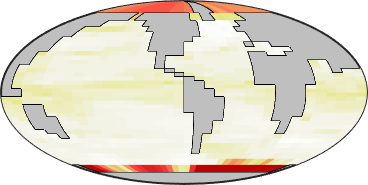
\includegraphics[width=0.95\linewidth]{/Users/ward/cgenie_output/BENW.worjh2.PO4FeTDTL_HYBRID_new.SPIN/figures/bio_fpart_POC_diff.png}
  \label{fig:dpCO2_2}
\end{subfigure}
%%%%%%%%%%%%%%%%%%%%%%%%%%%%%%%%%%%%%%%%%%%%%%%%%%%%%%%%%%%%
\\[+0.2cm]
%%%%%%%%%%%%%%%%%%%%%%%%%%%%%%%%%%%%%%%%%%%%%%%%%%%%%%%%%%%%
\begin{subfigure}{.49\textwidth}
  \centering
  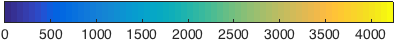
\includegraphics[width=0.95\linewidth]{/Users/ward/cgenie_output/BENW.worjh2.PO4FeTDTL_HYBRID_WF16_tgld_new.SPIN/figures/bio_fpart_POC_clrbr.png}
\end{subfigure}
\begin{subfigure}{.49\textwidth}
  \centering
  
\includegraphics[width=0.95\linewidth]{/Users/ward/cgenie_output/BENW.worjh2.PO4FeTDTL_HYBRID_new.SPIN/figures/bio_fpart_POC_clrbr_diff.png}
\end{subfigure}
%%%%%%%%%%%%%%%%%%%%%%%%%%%%%%%%%%%%%%%%%%%%%%%%%%%%%%%%%%%%
\\[+0.2cm]
%%%%%%%%%%%%%%%%%%%%%%%%%%%%%%%%%%%%%%%%%%%%%%%%%%%%%%%%%%%%
\begin{subfigure}{.33\textwidth}
  \centering
  \caption{POP production - BIOGEM}
  \includegraphics[width=0.95\linewidth]{/Users/ward/cgenie_output/BENW.worjh2.PO4FeTDTL_HYBRID_new.SPIN/figures/bio_fpart_POP.png}
  \label{fig:dpCO2_1}
\end{subfigure}%
\begin{subfigure}{.33\textwidth}
  \centering
  \caption{POP production - ECOGEM}
  \includegraphics[width=0.95\linewidth]{/Users/ward/cgenie_output/BENW.worjh2.PO4FeTDTL_HYBRID_WF16_tgld_new.SPIN/figures/bio_fpart_POP.png}
  \label{fig:dpCO2_2}
\end{subfigure}
\begin{subfigure}{.33\textwidth}
  \centering
  \caption{ECOGEM$\div$BIOGEM}
  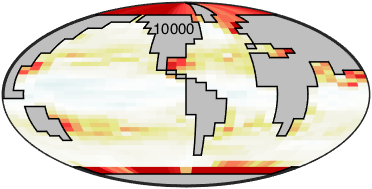
\includegraphics[width=0.95\linewidth]{/Users/ward/cgenie_output/BENW.worjh2.PO4FeTDTL_HYBRID_new.SPIN/figures/bio_fpart_POP_diff.png}
  \label{fig:dpCO2_2}
\end{subfigure}
%%%%%%%%%%%%%%%%%%%%%%%%%%%%%%%%%%%%%%%%%%%%%%%%%%%%%%%%%%%%
\\[+0.2cm]
%%%%%%%%%%%%%%%%%%%%%%%%%%%%%%%%%%%%%%%%%%%%%%%%%%%%%%%%%%%%
\begin{subfigure}{.49\textwidth}
  \centering
  
\includegraphics[width=0.95\linewidth]{/Users/ward/cgenie_output/BENW.worjh2.PO4FeTDTL_HYBRID_WF16_tgld_new.SPIN/figures/bio_fpart_POP_clrbr.png}
\end{subfigure}
\begin{subfigure}{.49\textwidth}
  \centering
  
\includegraphics[width=0.95\linewidth]{/Users/ward/cgenie_output/BENW.worjh2.PO4FeTDTL_HYBRID_new.SPIN/figures/bio_fpart_POP_clrbr_diff.png}
\end{subfigure}
%%%%%%%%%%%%%%%%%%%%%%%%%%%%%%%%%%%%%%%%%%%%%%%%%%%%%%%%%%%%
\\[+0.2cm]
%%%%%%%%%%%%%%%%%%%%%%%%%%%%%%%%%%%%%%%%%%%%%%%%%%%%%%%%%%%%
\begin{subfigure}{.33\textwidth}
  \centering
  \caption{POFe production - BIOGEM}
  \includegraphics[width=0.95\linewidth]{/Users/ward/cgenie_output/BENW.worjh2.PO4FeTDTL_HYBRID_new.SPIN/figures/bio_fpart_POFe.png}
  \label{fig:dpCO2_1}
\end{subfigure}%
\begin{subfigure}{.33\textwidth}
  \centering
  \caption{POFe production - ECOGEM}
  \includegraphics[width=0.95\linewidth]{/Users/ward/cgenie_output/BENW.worjh2.PO4FeTDTL_HYBRID_WF16_tgld_new.SPIN/figures/bio_fpart_POFe.png}
  \label{fig:dpCO2_2}
\end{subfigure}
\begin{subfigure}{.33\textwidth}
  \centering
  \caption{ECOGEM$\div$BIOGEM}
  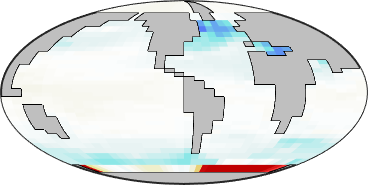
\includegraphics[width=0.95\linewidth]{/Users/ward/cgenie_output/BENW.worjh2.PO4FeTDTL_HYBRID_new.SPIN/figures/bio_fpart_POFe_diff.png}
  \label{fig:dpCO2_2}
\end{subfigure}
%%%%%%%%%%%%%%%%%%%%%%%%%%%%%%%%%%%%%%%%%%%%%%%%%%%%%%%%%%%%
\\[+0.2cm]
%%%%%%%%%%%%%%%%%%%%%%%%%%%%%%%%%%%%%%%%%%%%%%%%%%%%%%%%%%%%
\begin{subfigure}{.49\textwidth}
  \centering
  
\includegraphics[width=0.95\linewidth]{/Users/ward/cgenie_output/BENW.worjh2.PO4FeTDTL_HYBRID_WF16_tgld_new.SPIN/figures/bio_fpart_POFe_clrbr.png}
\end{subfigure}
\begin{subfigure}{.49\textwidth}
  \centering
  
\includegraphics[width=0.95\linewidth]{/Users/ward/cgenie_output/BENW.worjh2.PO4FeTDTL_HYBRID_new.SPIN/figures/bio_fpart_POFe_clrbr_diff.png}
\end{subfigure}
%%%%%%%%%%%%%%%%%%%%%%%%%%%%%%%%%%%%%%%%%%%%%%%%%%%%%%%%%%%%
\\[+0.2cm]
%%%%%%%%%%%%%%%%%%%%%%%%%%%%%%%%%%%%%%%%%%%%%%%%%%%%%%%%%%%%
\begin{subfigure}{.33\textwidth}
  \centering
  \caption{CaCO$_3$ production - BIOGEM}
  \includegraphics[width=0.95\linewidth]{/Users/ward/cgenie_output/BENW.worjh2.PO4FeTDTL_HYBRID_new.SPIN/figures/bio_fpart_CaCO3.png}
  \label{fig:dpCO2_1}
\end{subfigure}%
\begin{subfigure}{.33\textwidth}
  \centering
  \caption{CaCO$_3$ production - ECOGEM}
  \includegraphics[width=0.95\linewidth]{/Users/ward/cgenie_output/BENW.worjh2.PO4FeTDTL_HYBRID_WF16_tgld_new.SPIN/figures/bio_fpart_CaCO3.png}
  \label{fig:dpCO2_2}
\end{subfigure}
\begin{subfigure}{.33\textwidth}
  \centering
  \caption{ECOGEM$\div$BIOGEM}
  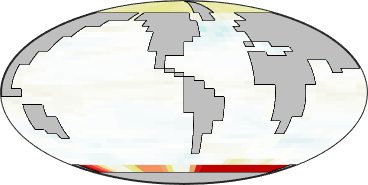
\includegraphics[width=0.95\linewidth]{/Users/ward/cgenie_output/BENW.worjh2.PO4FeTDTL_HYBRID_new.SPIN/figures/bio_fpart_CaCO3_diff.png}
  \label{fig:dpCO2_2}
\end{subfigure}
%%%%%%%%%%%%%%%%%%%%%%%%%%%%%%%%%%%%%%%%%%%%%%%%%%%%%%%%%%%%
\\[+0.2cm]
%%%%%%%%%%%%%%%%%%%%%%%%%%%%%%%%%%%%%%%%%%%%%%%%%%%%%%%%%%%%
\begin{subfigure}{.49\textwidth}
  \centering
  
\includegraphics[width=0.95\linewidth]{/Users/ward/cgenie_output/BENW.worjh2.PO4FeTDTL_HYBRID_WF16_tgld_new.SPIN/figures/bio_fpart_CaCO3_clrbr.png}
\end{subfigure}
\begin{subfigure}{.49\textwidth}
  \centering
  
\includegraphics[width=0.95\linewidth]{/Users/ward/cgenie_output/BENW.worjh2.PO4FeTDTL_HYBRID_new.SPIN/figures/bio_fpart_CaCO3_clrbr_diff.png}
\end{subfigure}
%%%%%%%%%%%%%%%%%%%%%%%%%%%%%%%%%%%%%%%%%%%%%%%%%%%%%%%%%%%%
\caption{Particulate matter production (and export from the surface layer). The right-hand column indicates the relative increase or decrease in ECOGEM, relative to BIOGEM.}
\label{fig:particulates}
\end{figure}

\clearpage
\subsubsection{Basin-averaged depth profiles}

In this section we present meridional depth distribution of key biogeochemical tracers, averaged across each of the three main ocean basins, as shown in Figure~\ref{fig:basins}. Figure~\ref{fig:basin_PO4} shows that the vertical distribution of dissolved phosphate is very similar between the two models, with EcoGENIE showing a slightly stronger sub-surface accumulation in the northern Indian Ocean. 

The vertical distributions shown in Figure~\ref{fig:basin_Fe} reveal that dissolved iron is lower throughout the ocean in EcoGENIE, relative to cGENIE, particularly below 1500 m. Differences are less obvious at intermediate depths. (Observations are currently too sparse to estimate reliable basin-scale distributions of dissolved iron; see Tagliabue 2016.)

Figure~\ref{fig:basin_DIC} shows that while cGENIE reproduces observed DIC distributions very well, EcoGENIE overestimates concentrations within the Indian and Pacific Oceans. The total oceanic DIC inventory increased by just under 2\% from 0.299 mol C in cGENIE to 0.304 in EcoGENIE (with a fixed atmospheric CO\(_{2}\) concentration of 278 ppm). Otherwise the two models show broadly similar distributions, with the most pronounced differences (as for PO$_4$) in the northern Indian Ocean.

Alkalinity (Figure 10), shows some pronounced differences between the two models, particularly in the Indian Ocean. In this region EcoGENIE shows excessive accumulation of alkalinity at $\sim$1000~m depth (this also occurs to a lesser degree in the north Pacific). The reason for this accumulation is that in the absence of a nitrogen cycle (and NO\(^{-}_{3}\) reduction) being included in the representation of global biogeochemical cycles adopted here, reduction of sulphate (to H\(_{2}\)S)  occurs as oxygen becomes depleted (Figure 11). The process of sulphate reduction  increases alkalinity of seawater. Further adjustment of the respiration of carbon in ECOGEM and hence the effective exported P:C Redfield ratio, and/or returning of the organic matter remineralization  profiles in BIOGEM [\textcolor{red}{Ridgwell et al., 2007}] would likely resolve this.

cGENIE reasonably captures the invasion of O$_2$ into the ocean interior through the Southern Ocean and North Atlantic (Figure 11),. These patterns are also seen in EcoGENIE, although concentrations in the far Northern deep ocean tend to be too low in the Indian and Pacific Oceans. Again, this is likely  a consequence of greater export and remineralisation of organic carbon in ECOGEM leading to more oxygen consumption as the intermediate depth regions of elevated PO$_4$ (Figure 7), DIC (Figure 9), and alkalinity (Figure 10), in the Indian and Pacific Oceans are also associated with water column anoxia (Figure 11),.


\begin{figure}[htp]
  \centering
  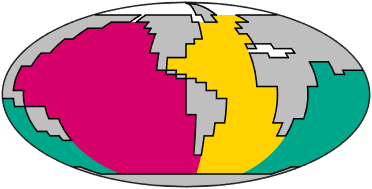
\includegraphics[width=0.5\linewidth]{/Users/ward/cgenie_output/EXAMPLE.worjh2.PO4FeTDTL_HYBRID.SPIN/figures/3basins.png}
\caption{Spatial definition of the three ocean basins used in Figures \ref{fig:basin_PO4} to \ref{fig:basin_O2}. Locations of the JGOFS time-series sites are indicated with blue dots.}
\label{fig:basins}
\end{figure}

\begin{figure}[htp]
\begin{subfigure}{.33\textwidth}
  \centering
  \caption{Atlantic PO$_4$ - WOA (2009)}
  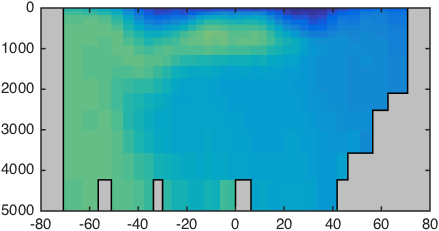
\includegraphics[width=0.95\linewidth]{/Users/ward/cgenie_output/WOA_2009_data/Atlantic_p_an_profile.png}
  \label{fig:nutrients1}
\end{subfigure}%
\begin{subfigure}{.33\textwidth}
  \centering
  \caption{Atlantic PO$_4$ - BIOGEM}
  \includegraphics[width=0.95\linewidth]{/Users/ward/cgenie_output/BENW.worjh2.PO4FeTDTL_HYBRID_new.SPIN/figures/Atlantic_ocn_PO4_profile.png}
  \label{fig:nutrients1}
\end{subfigure}%
\begin{subfigure}{.33\textwidth}
  \centering
  \caption{Atlantic PO$_4$ - ECOGEM}
  \includegraphics[width=0.95\linewidth]{/Users/ward/cgenie_output/BENW.worjh2.PO4FeTDTL_HYBRID_WF16_tgld_new.SPIN/figures/Atlantic_ocn_PO4_profile.png}
  \label{fig:nutrients2}
\end{subfigure}
\begin{subfigure}{.33\textwidth}
  \centering
  \caption{Indian PO$_4$ - WOA (2009)}
  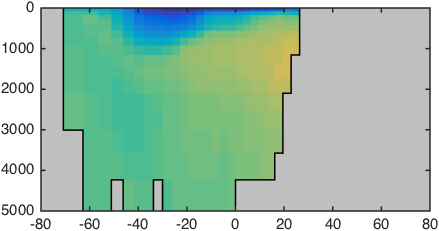
\includegraphics[width=0.95\linewidth]{/Users/ward/cgenie_output/WOA_2009_data/Indian_p_an_profile.png}
  \label{fig:nutrients1}
\end{subfigure}%
\begin{subfigure}{.33\textwidth}
  \centering
  \caption{Indian PO$_4$ - BIOGEM}
  \includegraphics[width=0.95\linewidth]{/Users/ward/cgenie_output/BENW.worjh2.PO4FeTDTL_HYBRID_new.SPIN/figures/Indian_ocn_PO4_profile.png}
  \label{fig:nutrients1}
\end{subfigure}%
\begin{subfigure}{.33\textwidth}
  \centering
  \caption{Indian PO$_4$ - ECOGEM}
  \includegraphics[width=0.95\linewidth]{/Users/ward/cgenie_output/BENW.worjh2.PO4FeTDTL_HYBRID_WF16_tgld_new.SPIN/figures/Indian_ocn_PO4_profile.png}
  \label{fig:nutrients2}
\end{subfigure}
\begin{subfigure}{.33\textwidth}
  \centering
  \caption{Pacific PO$_4$ - WOA (2009)}
  \includegraphics[width=0.95\linewidth]{/Users/ward/cgenie_output/WOA_2009_data/Pacific_p_an_profile.png}
  \label{fig:nutrients1}
\end{subfigure}%
\begin{subfigure}{.33\textwidth}
  \centering
  \caption{Pacific PO$_4$ - BIOGEM}
  \includegraphics[width=0.95\linewidth]{/Users/ward/cgenie_output/BENW.worjh2.PO4FeTDTL_HYBRID_new.SPIN/figures/Pacific_ocn_PO4_profile.png}
  \label{fig:nutrients1}
\end{subfigure}%
\begin{subfigure}{.33\textwidth}
  \centering
  \caption{Pacific PO$_4$ - ECOGEM}
  \includegraphics[width=0.95\linewidth]{/Users/ward/cgenie_output/BENW.worjh2.PO4FeTDTL_HYBRID_WF16_tgld_new.SPIN/figures/Pacific_ocn_PO4_profile.png}
  \label{fig:nutrients2}
\end{subfigure}
\\[+0.2cm]
\begin{subfigure}{.5\textwidth}
  \centering
  \includegraphics[width=0.95\linewidth]{/Users/ward/cgenie_output/BENW.worjh2.PO4FeTDTL_HYBRID_WF16_tgld_new.SPIN/figures/ocn_PO4_profile_clrbr.png}
\end{subfigure}
\caption{Basin-averaged meridional-depth distribution of phosphate.}
\label{fig:basin_PO4}
\end{figure}



\begin{figure}[htp]
\begin{subfigure}{.33\textwidth}
  \centering
  \caption{Atlantic dFe - BIOGEM}
  \includegraphics[width=0.95\linewidth]{/Users/ward/cgenie_output/BENW.worjh2.PO4FeTDTL_HYBRID_new.SPIN/figures/Atlantic_ocn_TDFe_profile.png}
  \label{fig:nutrients1}
\end{subfigure}%
\begin{subfigure}{.33\textwidth}
  \centering
  \caption{Atlantic dFe - ECOGEM}
  \includegraphics[width=0.95\linewidth]{/Users/ward/cgenie_output/BENW.worjh2.PO4FeTDTL_HYBRID_WF16_tgld_new.SPIN/figures/Atlantic_ocn_TDFe_profile.png}
  \label{fig:nutrients2}
\end{subfigure}
\begin{subfigure}{.33\textwidth}
  \centering
  \caption{Indian dFe - BIOGEM}
  \includegraphics[width=0.95\linewidth]{/Users/ward/cgenie_output/BENW.worjh2.PO4FeTDTL_HYBRID_new.SPIN/figures/Indian_ocn_TDFe_profile.png}
  \label{fig:nutrients1}
\end{subfigure}%
\begin{subfigure}{.33\textwidth}
  \centering
  \caption{Indian dFe - ECOGEM}
  \includegraphics[width=0.95\linewidth]{/Users/ward/cgenie_output/BENW.worjh2.PO4FeTDTL_HYBRID_WF16_tgld_new.SPIN/figures/Indian_ocn_TDFe_profile.png}
  \label{fig:nutrients2}
\end{subfigure}
\begin{subfigure}{.33\textwidth}
  \centering
  \caption{Pacific dFe - BIOGEM}
  \includegraphics[width=0.95\linewidth]{/Users/ward/cgenie_output/BENW.worjh2.PO4FeTDTL_HYBRID_new.SPIN/figures/Pacific_ocn_TDFe_profile.png}
  \label{fig:nutrients1}
\end{subfigure}%
\begin{subfigure}{.33\textwidth}
  \centering
  \caption{Pacific dFe - ECOGEM}
  \includegraphics[width=0.95\linewidth]{/Users/ward/cgenie_output/BENW.worjh2.PO4FeTDTL_HYBRID_WF16_tgld_new.SPIN/figures/Pacific_ocn_TDFe_profile.png}
  \label{fig:nutrients2}
\end{subfigure}
\\[+0.2cm]
\begin{subfigure}{.5\textwidth}
  \centering
  \includegraphics[width=0.95\linewidth]{/Users/ward/cgenie_output/BENW.worjh2.PO4FeTDTL_HYBRID_WF16_tgld_new.SPIN/figures/ocn_TDFe_profile_clrbr.png}
\end{subfigure}
\caption{Basin-averaged meridional-depth distribution of total dissolved iron (dFe).}
\label{fig:basin_Fe}
\end{figure}



\begin{figure}[htp]
\begin{subfigure}{.33\textwidth}
  \centering
  \caption{Atlantic DIC - GLODAP}
  \includegraphics[width=0.95\linewidth]{/Users/ward/cgenie_output/GLODAP_data/Atlantic_TCO2_profile.png}
  \label{fig:nutrients1}
\end{subfigure}%
\begin{subfigure}{.33\textwidth}
  \centering
  \caption{Atlantic DIC - BIOGEM}
  \includegraphics[width=0.95\linewidth]{/Users/ward/cgenie_output/BENW.worjh2.PO4FeTDTL_HYBRID_new.SPIN/figures/Atlantic_ocn_DIC_profile.png}
  \label{fig:nutrients1}
\end{subfigure}%
\begin{subfigure}{.33\textwidth}
  \centering
  \caption{Atlantic DIC - ECOGEM}
  \includegraphics[width=0.95\linewidth]{/Users/ward/cgenie_output/BENW.worjh2.PO4FeTDTL_HYBRID_WF16_tgld_new.SPIN/figures/Atlantic_ocn_DIC_profile.png}
  \label{fig:nutrients2}
\end{subfigure}
\begin{subfigure}{.33\textwidth}
  \centering
  \caption{Indian DIC - GLODAP}
  \includegraphics[width=0.95\linewidth]{/Users/ward/cgenie_output/GLODAP_data/Indian_TCO2_profile.png}
  \label{fig:nutrients1}
\end{subfigure}%
\begin{subfigure}{.33\textwidth}
  \centering
  \caption{Indian DIC - BIOGEM}
  \includegraphics[width=0.95\linewidth]{/Users/ward/cgenie_output/BENW.worjh2.PO4FeTDTL_HYBRID_new.SPIN/figures/Indian_ocn_DIC_profile.png}
  \label{fig:nutrients1}
\end{subfigure}%
\begin{subfigure}{.33\textwidth}
  \centering
  \caption{Indian DIC - ECOGEM}
  \includegraphics[width=0.95\linewidth]{/Users/ward/cgenie_output/BENW.worjh2.PO4FeTDTL_HYBRID_WF16_tgld_new.SPIN/figures/Indian_ocn_DIC_profile.png}
  \label{fig:nutrients2}
\end{subfigure}
\begin{subfigure}{.33\textwidth}
  \centering
  \caption{Pacific DIC - GLODAP}
  \includegraphics[width=0.95\linewidth]{/Users/ward/cgenie_output/GLODAP_data/Pacific_TCO2_profile.png}
  \label{fig:nutrients1}
\end{subfigure}%
\begin{subfigure}{.33\textwidth}
  \centering
  \caption{Pacific DIC - BIOGEM}
  \includegraphics[width=0.95\linewidth]{/Users/ward/cgenie_output/BENW.worjh2.PO4FeTDTL_HYBRID_new.SPIN/figures/Pacific_ocn_DIC_profile.png}
  \label{fig:nutrients1}
\end{subfigure}%
\begin{subfigure}{.33\textwidth}
  \centering
  \caption{Pacific DIC - ECOGEM}
  \includegraphics[width=0.95\linewidth]{/Users/ward/cgenie_output/BENW.worjh2.PO4FeTDTL_HYBRID_WF16_tgld_new.SPIN/figures/Pacific_ocn_DIC_profile.png}
  \label{fig:nutrients2}
\end{subfigure}
\\[+0.2cm]
\begin{subfigure}{.5\textwidth}
  \centering
  \includegraphics[width=0.95\linewidth]{/Users/ward/cgenie_output/BENW.worjh2.PO4FeTDTL_HYBRID_WF16_tgld_new.SPIN/figures/ocn_DIC_profile_clrbr.png}
\end{subfigure}
\caption{Basin-averaged meridional-depth distribution of DIC.}
\label{fig:basin_DIC}
\end{figure}


\begin{figure}[htp]
\begin{subfigure}{.33\textwidth}
  \centering
  \caption{Atlantic ALK - GLODAP}
  \includegraphics[width=0.95\linewidth]{/Users/ward/cgenie_output/GLODAP_data/Atlantic_PALK_profile.png}
  \label{fig:nutrients1}
\end{subfigure}%
\begin{subfigure}{.33\textwidth}
  \centering
  \caption{Atlantic Alkalinity - BIOGEM}
  \includegraphics[width=0.95\linewidth]{/Users/ward/cgenie_output/BENW.worjh2.PO4FeTDTL_HYBRID_new.SPIN/figures/Atlantic_ocn_ALK_profile.png}
  \label{fig:nutrients1}
\end{subfigure}%
\begin{subfigure}{.33\textwidth}
  \centering
  \caption{Atlantic Alkalinity - ECOGEM}
  \includegraphics[width=0.95\linewidth]{/Users/ward/cgenie_output/BENW.worjh2.PO4FeTDTL_HYBRID_WF16_tgld_new.SPIN/figures/Atlantic_ocn_ALK_profile.png}
  \label{fig:nutrients2}
\end{subfigure}
\begin{subfigure}{.33\textwidth}
  \centering
  \caption{Indian ALK - GLODAP}
  \includegraphics[width=0.95\linewidth]{/Users/ward/cgenie_output/GLODAP_data/Indian_PALK_profile.png}
  \label{fig:nutrients1}
\end{subfigure}%
\begin{subfigure}{.33\textwidth}
  \centering
  \caption{Indian Alkalinity - BIOGEM}
  \includegraphics[width=0.95\linewidth]{/Users/ward/cgenie_output/BENW.worjh2.PO4FeTDTL_HYBRID_new.SPIN/figures/Indian_ocn_ALK_profile.png}
  \label{fig:nutrients1}
\end{subfigure}%
\begin{subfigure}{.33\textwidth}
  \centering
  \caption{Indian Alkalinity - ECOGEM}
  \includegraphics[width=0.95\linewidth]{/Users/ward/cgenie_output/BENW.worjh2.PO4FeTDTL_HYBRID_WF16_tgld_new.SPIN/figures/Indian_ocn_ALK_profile.png}
  \label{fig:nutrients2}
\end{subfigure}
\begin{subfigure}{.33\textwidth}
  \centering
  \caption{Pacific ALK - GLODAP}
  \includegraphics[width=0.95\linewidth]{/Users/ward/cgenie_output/GLODAP_data/Pacific_PALK_profile.png}
  \label{fig:nutrients1}
\end{subfigure}%
\begin{subfigure}{.33\textwidth}
  \centering
  \caption{Pacific Alkalinity - BIOGEM}
  \includegraphics[width=0.95\linewidth]{/Users/ward/cgenie_output/BENW.worjh2.PO4FeTDTL_HYBRID_new.SPIN/figures/Pacific_ocn_ALK_profile.png}
  \label{fig:nutrients1}
\end{subfigure}%
\begin{subfigure}{.33\textwidth}
  \centering
  \caption{Pacific Alkalinity - ECOGEM}
  \includegraphics[width=0.95\linewidth]{/Users/ward/cgenie_output/BENW.worjh2.PO4FeTDTL_HYBRID_WF16_tgld_new.SPIN/figures/Pacific_ocn_ALK_profile.png}
  \label{fig:nutrients2}
\end{subfigure}
\\[+0.2cm]
\begin{subfigure}{.5\textwidth}
  \centering
  \includegraphics[width=0.95\linewidth]{/Users/ward/cgenie_output/BENW.worjh2.PO4FeTDTL_HYBRID_WF16_tgld_new.SPIN/figures/ocn_ALK_profile_clrbr.png}
\end{subfigure}
\caption{Basin-averaged meridional-depth distribution of alkalinity.}
\label{fig:basin_ALK}
\end{figure}



\begin{figure}[htp]
\begin{subfigure}{.33\textwidth}
  \centering
  \caption{Atlantic O$_2$ - WOA (2009)}
  \includegraphics[width=0.95\linewidth]{/Users/ward/cgenie_output/WOA_2009_data/Atlantic_o_an_profile.png}
  \label{fig:nutrients1}
\end{subfigure}%
\begin{subfigure}{.33\textwidth}
  \centering
  \caption{Atlantic O$_2$ - BIOGEM}
  \includegraphics[width=0.95\linewidth]{/Users/ward/cgenie_output/BENW.worjh2.PO4FeTDTL_HYBRID_new.SPIN/figures/Atlantic_ocn_O2_profile.png}
  \label{fig:nutrients1}
\end{subfigure}%
\begin{subfigure}{.33\textwidth}
  \centering
  \caption{Atlantic O$_2$ - ECOGEM}
  \includegraphics[width=0.95\linewidth]{/Users/ward/cgenie_output/BENW.worjh2.PO4FeTDTL_HYBRID_WF16_tgld_new.SPIN/figures/Atlantic_ocn_O2_profile.png}
  \label{fig:nutrients2}
\end{subfigure}
\begin{subfigure}{.33\textwidth}
  \centering
  \caption{Indian O$_2$ - WOA (2009)}
  \includegraphics[width=0.95\linewidth]{/Users/ward/cgenie_output/WOA_2009_data/Indian_o_an_profile.png}
  \label{fig:nutrients1}
\end{subfigure}%
\begin{subfigure}{.33\textwidth}
  \centering
  \caption{Indian O$_2$ - BIOGEM}
  \includegraphics[width=0.95\linewidth]{/Users/ward/cgenie_output/BENW.worjh2.PO4FeTDTL_HYBRID_new.SPIN/figures/Indian_ocn_O2_profile.png}
  \label{fig:nutrients1}
\end{subfigure}%
\begin{subfigure}{.33\textwidth}
  \centering
  \caption{Indian O$_2$ - ECOGEM}
  \includegraphics[width=0.95\linewidth]{/Users/ward/cgenie_output/BENW.worjh2.PO4FeTDTL_HYBRID_WF16_tgld_new.SPIN/figures/Indian_ocn_O2_profile.png}
  \label{fig:nutrients2}
\end{subfigure}
\begin{subfigure}{.33\textwidth}
  \centering
  \caption{Pacific O$_2$ - WOA (2009)}
  \includegraphics[width=0.95\linewidth]{/Users/ward/cgenie_output/WOA_2009_data/Pacific_o_an_profile.png}
  \label{fig:nutrients1}
\end{subfigure}%
\begin{subfigure}{.33\textwidth}
  \centering
  \caption{Pacific O$_2$ - BIOGEM}
  \includegraphics[width=0.95\linewidth]{/Users/ward/cgenie_output/BENW.worjh2.PO4FeTDTL_HYBRID_new.SPIN/figures/Pacific_ocn_O2_profile.png}
  \label{fig:nutrients1}
\end{subfigure}%
\begin{subfigure}{.33\textwidth}
  \centering
  \caption{Pacific O$_2$ - ECOGEM}
  \includegraphics[width=0.95\linewidth]{/Users/ward/cgenie_output/BENW.worjh2.PO4FeTDTL_HYBRID_WF16_tgld_new.SPIN/figures/Pacific_ocn_O2_profile.png}
  \label{fig:nutrients2}
\end{subfigure}
\\[+0.2cm]
\begin{subfigure}{.5\textwidth}
  \centering
  \includegraphics[width=0.95\linewidth]{/Users/ward/cgenie_output/BENW.worjh2.PO4FeTDTL_HYBRID_WF16_tgld_new.SPIN/figures/ocn_O2_profile_clrbr.png}
\end{subfigure}
\caption{Basin-averaged meridional-depth distribution of dissolved oxygen.}
\label{fig:basin_O2}
\end{figure}

\clearpage
\subsubsection{Time-series}

Figures~\ref{fig:jgofs_po4} and~\ref{fig:jgofs_fe} we compare the seasonal cycles of surface nutrients (phosphate and iron) at nine Joint Global Ocean Flux Study (JGOFS) sites.

\begin{figure}[htbp]
\begin{center}
\includegraphics[width=16cm]{/Users/ward/cgenie_output/BENW.worjh2.PO4FeTDTL_HYBRID_WF16_tgld_final.SPIN/figures/JGOFS_Phosphate.png}
\caption{Annual cycle of surface PO$_4$ at 9 time-series sites in cGENIE and EcoGENIE. Red dots indicate climatological observations, while the lines represent modelled surface PO$_4$concentrations. Locations of the time-series are indicated in Figure~\ref{fig:basins}.}
\label{fig:jgofs_po4}
\end{center}
\end{figure}


\begin{figure}[htbp]
\begin{center}
\includegraphics[width=16cm]{/Users/ward/cgenie_output/BENW.worjh2.PO4FeTDTL_HYBRID_WF16_tgld_final.SPIN/figures/JGOFS_Iron.png}
\caption{Annual cycle of surface dissolved iron at 9 time-series sites in cGENIE and EcoGENIE. Red dots indicate climatological observations, while the 
lines represent modelled surface iron concentrations. Locations of the time-series are indicated in Figure~\ref{fig:basins}.}
\label{fig:jgofs_fe}
\end{center}
\end{figure}

\clearpage
\subsection{Ecological variables}

Moving on from the core components that are common to both models, we present a range of ecological variables that are exclusive to ECOGEM (and  coupled as part of EcoGENIE). As before, we begin by presenting the annual mean global distributions in the ocean surface layer, comparing total chlorophyll and primary production to satellite-derived estimates (Figure~\ref{fig:chl_prpr}). We then look in more detail at the community composition, with Figure~\ref{fig:surf_sizefrac} showing the carbon biomass within each plankton population. Figure~\ref{fig:surf_sizefrac_limitation} then shows the degree of nutrient limitation within each phytoplankton population. Finally, in Figure~\ref{fig:jgofs_chl}, we show the seasonal cycle of community and population level chlorophyll at each of the nine JGOFS time-series sites.

\subsubsection{Global surface values}

Figure~\ref{fig:chl_prpr} reveals that ECOGEM shows some limited agreement with the satellite-derived estimate of global chlorophyll. As expected, chlorophyll biomass is elevated in the high-latitude oceans relative to lower latitudes. The sub-tropical gyres show low biomass, but the distinction with higher latitudes is not as clear as in the satellite estimate. The model also shows a clear lack of chlorophyll in equatorial and coastal upwelling regions, relative to the satellite estimate. The model predicts higher chlorophyll concentrations in the Southern Ocean, although this may, in part, be related to the satellite algorithm overestimating concentrations in these regions \citep{Dierssen:2010}.

Modelled primary production correctly increases from the oligotrophic gyres towards high latitudes and upwelling regions, but variability is much lower than in the satellite estimate. Specifically, the model and satellite estimates yield broadly similar estimates in the oligotrophic gyres, but the model does not attain the high values seen at higher latitudes and in coastal areas.

\begin{figure}[htbp]
\begin{subfigure}{.5\textwidth}
\centering
  \caption{SeaWiFS Chlorophyll}
\includegraphics[width=0.95\linewidth]{/Users/ward/cgenie_output/Satellite_data/SeaWiFS_on_GEnIE.png}
\end{subfigure}%
\begin{subfigure}{.5\textwidth}
\centering
  \caption{ECOGEM Chlorophyll}
\includegraphics[width=0.95\linewidth]{/Users/ward/cgenie_output/BENW.worjh2.PO4FeTDTL_HYBRID_WF16_tgld_new.SPIN/figures/Surface_Chl_Biomass.png}
\end{subfigure}%
\\[+0.2cm]
\begin{subfigure}{.5\textwidth}
  \centering
  \includegraphics[width=0.95\linewidth]{/Users/ward/cgenie_output/BENW.worjh2.PO4FeTDTL_HYBRID_WF16_tgld_new.SPIN/figures/Surface_Chl_Biomass_clrbar.png}
\end{subfigure}
%%%%%
\begin{subfigure}{.5\textwidth}
\centering
  \caption{\citet{Yool:2013a} Pr. Production}
\includegraphics[width=0.95\linewidth]{/Users/ward/cgenie_output/Satellite_data/Composite_PP_on_GEnIE.png}
\end{subfigure}%
\begin{subfigure}{.5\textwidth}
\centering
  \caption{ECOGEM Pr.  Production}
\includegraphics[width=0.95\linewidth]{/Users/ward/cgenie_output/BENW.worjh2.PO4FeTDTL_HYBRID_WF16_tgld_new.SPIN/figures/PrimaryProdn.png}
\end{subfigure}%
\\[+0.2cm]
\begin{subfigure}{.5\textwidth}
  \centering
  \includegraphics[width=0.95\linewidth]{/Users/ward/cgenie_output/BENW.worjh2.PO4FeTDTL_HYBRID_WF16_tgld_new.SPIN/figures/PrimaryProdn_clrbar.png}
\end{subfigure}
\caption{Satellite-derived (left) and modelled (right) surface chlorophyll~\textit{a} concentration and depth-integrated primary production. The satellite-derived estimate of primary production is a composite of three products \citep{Behrenfeld:1997,Carr:2006,Westberry:2008}, as in \citet[][Figure~12]{Yool:2013a}.}
\label{fig:chl_prpr}
\end{figure}

Figure~\ref{fig:surf_sizefrac} shows the modelled carbon biomass concentrations in the surface layer, for each modelled plankton population. The smallest (0.6 $\mu$m) phytoplankton size class is evenly distributed in the low-latitude oceans between 40$^\circ$ N and S, but is largely absent nearer to the poles. The 1.9 $\mu$m phytoplankton size class is similarly ubiquitous at low latitudes, albeit with somewhat higher biomass, and its range extends much further towards the poles. With increasing size, the larger phytoplankton are increasingly restricted to highly productive areas, such as the sub-polar gyres and upwelling zones. 

Perhaps as expected, zooplankton size classes tend to mirror the biogeography of their phytoplankton prey. The smallest (1.9 $\mu$m) size class is found primarily at low latitudes, although a highly variable population is found at higher latitudes. This population is presumably supported by grazing on the larger 6 $\mu$m size class (with very low efficiency dictated by the unfavourable predator-prey length ratio). Larger zooplankton size classes follow a similar pattern to the phytoplankton, moving from a cosmopolitan but homogenous distribution in the smaller size classes, towards spatially more variable distributions among the larger organisms.

\begin{figure}[htbp]
\begin{subfigure}{.66\textwidth}
  \centering
\includegraphics[width=0.95\linewidth]{/Users/ward/cgenie_output/BENW.worjh2.PO4FeTDTL_HYBRID_WF16_tgld_new.SPIN/figures/SizeClass_C_Biomass.png}
\end{subfigure} 
\\[+0.2cm]
\begin{subfigure}{.66\textwidth}
  \centering
\includegraphics[width=0.95\linewidth]{/Users/ward/cgenie_output/BENW.worjh2.PO4FeTDTL_HYBRID_WF16_tgld_new.SPIN/figures/SizeClass_C_Biomass_clrbar.png}
\end{subfigure}
\caption{Surface concentrations of carbon biomass in each population.}
\label{fig:surf_sizefrac}
\end{figure}

The degree of nutrient limitation within each phytoplankton size class is shown in Figure~\ref{fig:surf_sizefrac_limitation}. The two-dimensional colour-scale indicates decreasing iron limitation from left to right, and decreasing phosphorus limitation from bottom to top. White is therefore nutrient replete, blue is phosphorus limited, red is iron limited, and magenta is phosphorus-iron co-limited. The figure demonstrates that the smallest size class is not nutrient limited in any region. The increasing saturation of the colour scale in larger size classes indicates an increasing degree of nutrient limitation. As expected, nutrient limitation is strongest in the highly stratified low latitudes. A stronger vertical supply of nutrients at higher latitudes is associated with weaker nutrient limitation, although nutrient limitation is still significant among the larger size classes. Consistent with observations \citep{Moore:2013}, phosphorus limitation is restricted is restricted to low latitudes. Iron limitation dominates in high latitude regions. Among the larger size classes the upwelling zones appear to be characterised by iron-phosphorus co-limitation.

\begin{figure}[htbp]
\begin{subfigure}{.33\textwidth}
  \centering
\includegraphics[width=0.95\linewidth]{/Users/ward/cgenie_output/BENW.worjh2.PO4FeTDTL_HYBRID_WF16_tgld_new.SPIN/figures/SizeClass_Limitation.png}
\end{subfigure}
\begin{subfigure}{.25\textwidth}
  \centering
\includegraphics[width=0.95\linewidth]{/Users/ward/cgenie_output/BENW.worjh2.PO4FeTDTL_HYBRID_WF16_tgld_new.SPIN/figures/SizeClass_Limitation_clrbar.png}
\end{subfigure}
\caption{Nutrient limitation in each phytoplankton population. The two-dimensional colour-scale indicates decreasing phosphorus limitation from left to right, and decreasing iron limitation from bottom to top. White is therefore nutrient replete, blue is phosphorus limited, red is iron limited, and magenta is phosphorus-iron co-limited.}
\label{fig:surf_sizefrac_limitation}
\end{figure}

\clearpage
\subsubsection{Time-series}

The seasonal cycles of phytoplankton chlorophyll~\textit{a} are compared to time-series observations in Figure~\ref{fig:jgofs_chl}. The modelled total chlorophyll concentrations (black lines) track the observed concentrations (red dots) reasonably well at most sites, and perhaps better than might be expected from the comparison to satellite data in Figure~\ref{fig:chl_prpr}. The modelled surface chlorophyll concentration is probably too low in the equatorial Pacific, while the spring bloom occurs one to two months earlier than was seen during the North Atlantic Bloom Experiment. 

\begin{figure}[htbp]
\begin{center}
\includegraphics[width=16cm]{/Users/ward/cgenie_output/BENW.worjh2.PO4FeTDTL_HYBRID_WF16_tgld_final.SPIN/figures/JGOFS_Chlorophyll.png}
\caption{Annual cycle of surface chlorophyll~\textit{a} at nine JGOFS time-series sites. Red dots indicate climatological observations, while the black lines represents modelled total surface chlorophyll~\textit{a}. Coloured lines represent chlorophyll~\textit{a} in individual size classes (blue = small, red = large). Locations of the time-series are indicated in Figure~\ref{fig:basins}.}
\label{fig:jgofs_chl}
\end{center}
\end{figure}

\begin{figure}[htbp]
\begin{center}
\includegraphics[width=16cm]{/Users/ward/cgenie_output/BENW.worjh2.PO4FeTDTL_HYBRID_WF16_tgld_final.SPIN/figures/JGOFS_PrProduction.png}
\caption{Annual cycle of surface primary production at nine JGOFS time-series sites. Red dots indicate climatological observations, while the black lines represents modelled total primary production. Locations of the time-series are indicated in Figure~\ref{fig:basins}.}
\label{fig:jgofs_chl}
\end{center}
\end{figure}

\clearpage
\subsubsection{cGENIE vs. EcoGENIE}

Figure~\ref{fig:taylor} is a Taylor diagram comparing the two models in terms of their correlation to observations and their standard deviations, relative to observations. A perfect model would be located at the middle of the bottom axis, with a correlation coefficient of 1.0 and a normalised standard deviation of 1.0. The closer a model is to this ideal point, the better a representation of the data it provides. Figure~\ref{fig:taylor} shows that EcoGENIE is located further from the ideal point than cGENIE, in terms of oxygen, alkalinity, phosphate, and DIC. The new model seems to provide a universally worse representation of global ocean biogeochemistry. This is perhaps not surprising, given that the BIOGEM component of cGENIE has at various times formally (e.g.  \citep{Ridgwell:2007}.) or informally (e.g. \textcolor{red}{REF})  systematically tuned to match the observation data. EcoGENIE has not yet been optimised in this way.

\begin{figure}[htbp]
\begin{center}
\includegraphics[width=8cm]{/Users/ward/GoogleDrive/DarwinianGenie/Figures/Taylor_diagrams/Taylor.png}
\caption{Taylor diagram comparing cGENIE and EcoGENIE to annual mean observation fields.}
\label{fig:taylor}
\end{center}
\end{figure}

%%%%%%%%%%%%%%%%%%%%%%%%%%%%%%%%%%%%%%%%%%%%%%%%%%%%%%%%%%%%%%%%%%%%%%%
\clearpage
\section{Discussion}

The marine ecosystem is a central component of the Earth system, harnessing solar energy to sustain the biogeochemical cycling of elements between dissolved inorganic nutrients, living biomass and decaying organic matter. The interaction of these components with the global carbon cycle is critical to our interpretation of past, present and future climates, and has motivated the development of a wide range of models. These can be placed on a spectrum of increasing complexity, from simple and computationally efficient box models to fully coupled Earth system models with extremely large computational overheads. 

cGENIE is a model of intermediate complexity on this spectrum. It has been designed to allow rapid model evaluation while at the same time retaining somewhat realistic global dynamics that facilitate comparison with observations. With this goal in mind, the biological pump was parameterised as a simple vertical flux defined as a function of environmental conditions \citep{Ridgwell:2007}. This simplicity is well suited to questions concerning the interactions of marine biogeochemistry and climate, but at the same time precludes any investigation of the role of ecological interactions with the broader Earth system.

Here we have presented an ecological extension to cGENIE that opens up this area of investigation. The ecological model is rooted in size-dependent physiological and ecological constraints \citep{Ward:2012}. The ecophysiological parameters are relatively well constrained by observations, even in comparison to simpler ecosystem models that are based on much more aggregated functional groups \citep{Anderson:2005,Litchman:2007}. The size-based formulation has the additional benefit of linking directly to functional aspects of the ecosystem, such as food-web structure and particle sinking \citep{Ward:2016}. 

The aim of this paper is to provide a detailed description of the new ecological component. It is clear from Figure~\ref{fig:taylor} that the switch from the parameterised biological pump to the explicit ecological model has led to a deterioration in the overall ability of cGENIE to reproduce the global distributions of important biogeochemical tracers. This is an acceptable outcome, as our goal here is simply to provide a full description of the new model. Given that the original model was calibrated to the observations in question \citep{Ridgwell:2007}, that process will need to be repeated for the new model before any sort of objective comparison can be made.

Despite a slight overall deterioration in terms of model-observation misfit, the biogeochemical components of the model retain the key features that should be expected. At the same time, the ecological community conforms to expectations in terms of standing stocks and fluxes, both in terms of large-scale spatial distributions, and the seasonal cycles at specific locations. Overall patterns of community structure and physiological limitation also follow expectations based on observations and theory. 

As presented, the model is limited to three limiting resources (light, phosphorus, and iron) and two plankton functional types (phytoplankton and zooplankton). We have written the model equations to facilitate the extension of the model to include additional components. In particular, the model capabilities can be extended by enabling silicon and nitrogen limitation, leveraging the silicon and nitrogen cycles already present in BIOGEM \citep{Monteiro:2012}. Adding these nutrients will enable the addition of diatoms and diazotrophs, which are both likely to be important factors affecting the strength of the long-term biological pump \citep{Tyrrell:1999,Armstrong:2002}.

%In its presented configuration, GEnIE has a very coarse spatial resolution. Horizontal resolution is no less than 10 degrees, and the surface layer has a fixed thickness of $\sim$80~m. In addition, all phytoplankton growth is restricted to this surface layer. On the one hand this configuration enables rapid integration of the model, but on the other, it precludes the accurate representation of planktonic environment. The importance of this crude structure is not yet known in terms of the ecological dynamics, so it will be helpful in future to examine the model in more realistic configurations. Key adaptations would be the adoption of a fine-scale model grid \citep{}, and the extension of the model to allow plankton growth deeper in the water column.

%%%%%%%%%%%%%%%%%%%%%%%%%%%%%%%%%%%%%%%%%%%%%%%%%%%%%%%%%%%%%%%%%%%%%%%

\section{Code availability}  %% \conclusions[modified heading if necessary]

The model code and user instructions can be found at \href{http://www.seao2.info/mycgenie.html}{http://www.seao2.info/mycgenie.html}.

SVN number ????

%%%%%%%%%%%%%%%%%%%%%%%%%%%%%%%%%%%%%%%%%%%%%%%%%%%%%%%%%%%%%%%%%%%%%%%

%\appendix




\begin{acknowledgements}
This work was supported by the European Research Council `PALEOGENiE' project (ERC-2013-CoG-617313). BAW thanks the Marine Systems Modelling group at the National Oceanography Centre, Southampton.
\end{acknowledgements}


%% REFERENCES

%% The reference list is compiled as follows:

\clearpage

%% Since the Copernicus LaTeX package includes the BibTeX style file copernicus.bst,
%% authors experienced with BibTeX only have to include the following two lines:
%%

\bibliography{biblio1}
\bibliographystyle{copernicus}
%% \bibliographystyle{copernicus}
%% \bibliography{example.bib}
%%
%% URLs and DOIs can be entered in your BibTeX file as:
%%
%% URL = {http://www.xyz.org/~jones/idx_g.htm}
%% DOI = {10.5194/xyz}


%% LITERATURE CITATIONS
%%
%% command                        & example result
%% \citet{jones90}|               & Jones et al. (1990)
%% \citep{jones90}|               & (Jones et al., 1990)
%% \citep{jones90,jones93}|       & (Jones et al., 1990, 1993)
%% \citep[p.~32]{jones90}|        & (Jones et al., 1990, p.~32)
%% \citep[e.g.,][]{jones90}|      & (e.g., Jones et al., 1990)
%% \citep[e.g.,][p.~32]{jones90}| & (e.g., Jones et al., 1990, p.~32)
%% \citeauthor{jones90}|          & Jones et al.
%% \citeyear{jones90}|            & 1990



%% FIGURES

%% ONE-COLUMN FIGURES

%%f
%
%%% TWO-COLUMN FIGURES
%
%%f
%\begin{figure*}[t]
%\includegraphics[width=12cm]{FILE NAME}
%\caption{TEXT}
%\end{figure*}
%
%
%%% TABLES
%%%
%%% The different columns must be seperated with a & command and should
%%% end with \\ to identify the column brake.
%
%%% ONE-COLUMN TABLE
%
%%t
%\begin{table}[t]
%\caption{TEXT}
%\begin{tabular}{column = lcr}
%\tophline
%
%\middlehline
%
%\bottomhline
%\end{tabular}
%\belowtable{} % Table Footnotes
%\end{table}
%
%%% TWO-COLUMN TABLE
%
%%t
%\begin{table*}[t]
%\caption{TEXT}
%\begin{tabular}{column = lcr}
%\tophline
%
%\middlehline
%
%\bottomhline
%\end{tabular}
%\belowtable{} % Table Footnotes
%\end{table*}
%
%
%%% NUMBERING OF FIGURES AND TABLES
%%%
%%% If figures and tables must be numbered 1a, 1b, etc. the following command
%%% should be inserted before the begin{} command.
%
%\addtocounter{figure}{-1}\renewcommand{\thefigure}{\arabic{figure}a}
%
%
%%% MATHEMATICAL EXPRESSIONS
%
%%% All papers typeset by Copernicus Publications follow the math typesetting regulations
%%% given by the IUPAC Green Book (IUPAC: Quantities, Units and Symbols in Physical Chemistry,
%%% 2nd Edn., Blackwell Science, available at: http://old.iupac.org/publications/books/gbook/green_book_2ed.pdf, 1993).
%%%
%%% Physical quantities/variables are typeset in italic font (t for time, T for Temperature)
%%% Indices which are not defined are typeset in italic font (x, y, z, a, b, c)
%%% Items/objects which are defined are typeset in roman font (Car A, Car B)
%%% Descriptions/specifications which are defined by itself are typeset in roman font (abs, rel, ref, tot, net, ice)
%%% Abbreviations from 2 letters are typeset in roman font (RH, LAI)
%%% Vectors are identified in bold italic font using \vec{x}
%%% Matrices are identified in bold roman font
%%% Multiplication signs are typeset using the LaTeX commands \times (for vector products, grids, and exponential notations) or \cdot
%%% The character * should not be applied as mutliplication sign
%
%
%%% EQUATIONS
%
%%% Single-row equation
%
%\begin{equation}
%
%\end{equation}
%
%%% Multiline equation
%
%\begin{align}
%& 3 + 5 = 8\\
%& 3 + 5 = 8\\
%& 3 + 5 = 8
%\end{align}
%
%
%%% MATRICES
%
%\begin{matrix}
%x & y & z\\
%x & y & z\\
%x & y & z\\
%\end{matrix}
%
%
%%% ALGORITHM
%
%\begin{algorithm}
%\caption{�}
%\label{a1}
%\begin{algorithmic}
%�
%\end{algorithmic}
%\end{algorithm}
%
%
%%% CHEMICAL FORMULAS AND REACTIONS
%
%%% For formulas embedded in the text, please use \chem{}
%
%%% The reaction environment creates labels including the letter R, i.e. (R1), (R2), etc.
%
%\begin{reaction}
%%% \rightarrow should be used for normal (one-way) chemical reactions
%%% \rightleftharpoons should be used for equilibria
%%% \leftrightarrow should be used for resonance structures
%\end{reaction}
%
%
%%% PHYSICAL UNITS
%%%
%%% Please use \unit{} and apply the exponential notation


\end{document}
